\documentclass[12pt,a4paper]{article}
\usepackage[utf8]{inputenc}
\usepackage[top=3.0cm,bottom=3.0cm,left=4.0cm,right=3.0cm,footskip=1.2cm,headheight=15pt]{geometry}
\usepackage{times}
\usepackage{graphicx}
\usepackage{setspace}
\usepackage{tabularx}
\usepackage{array}
\usepackage{enumitem}
\usepackage{fancyhdr}
\usepackage{xurl}
\usepackage{hyperref}
\usepackage{caption}

\hypersetup{
    colorlinks=false,
    pdfborder={0 0 0}
}

\onehalfspacing
\setlength{\parindent}{1.2cm}
\setlength{\parskip}{0pt}

% Page number style matching Azziz template: bottom-right
\pagestyle{fancy}
\fancyhf{}
\renewcommand{\headrulewidth}{0pt}
\fancyfoot[R]{\thepage}

\renewcommand{\figurename}{Gambar}
\renewcommand{\tablename}{Tabel}
\renewcommand{\thefigure}{3.\arabic{figure}}
\renewcommand{\thetable}{3.\arabic{table}}

\begin{document}

% ==================== COVER (Page 1 - No Page Number) ====================
\begin{titlepage}
    \thispagestyle{empty}
    \begin{center}
        {\bfseries\large LAPORAN KERJA PRAKTIK\par}
        \vspace{1.2cm}
        {\bfseries\large PENGUJIAN PERANGKAT LUNAK BERBASIS OTOMASI SEBAGAI QUALITY ASSURANCE AUTOMATION ENGINEER\par}
        \vspace{0.4cm}
        {\bfseries\large PT XLSMART Telecom Sejahtera Tbk\par}

        \vspace{2.2cm}
        
\includegraphics[width=3.4cm]{telkom_logo.png}

        \vspace{2.5cm}
        {\bfseries\normalsize Oleh :\par}
        \vspace{0.3cm}
        {\normalsize Daniandra Prayudisty Ilham \quad 103012300052\par}

        \vfill
        {\bfseries\normalsize
            PROGRAM STUDI S1 INFORMATIKA\par
            FAKULTAS INFORMATIKA\par
            UNIVERSITAS TELKOM\par
            BANDUNG\par
            2026\par
        }
    \end{center}
\end{titlepage}

% ==================== LEMBAR PENGESAHAN (Page ii) ====================
\clearpage
\pagenumbering{roman}
\setcounter{page}{2}

\begin{center}
    {\bfseries\large LEMBAR PENGESAHAN\par}
    \vspace{0.6cm}
    {\bfseries\large LAPORAN KERJA PRAKTIK\par}
    \vspace{0.4cm}
    {\bfseries\normalsize PENGUJIAN PERANGKAT LUNAK BERBASIS OTOMASI SEBAGAI QUALITY ASSURANCE AUTOMATION ENGINEER\par}
    \vspace{0.2cm}
    {\bfseries\normalsize PADA PERUSAHAAN/INSTANSI PT XLSMART TELECOM SEJAHTERA TBK\par}
    \vspace{0.5cm}
    {\normalsize Sebagai salah satu syarat dalam melaksanakan perkuliahan Mata Kuliah Kerja Praktik\par}
    \vspace{0.5cm}
    {\normalsize Oleh :\par}
    \vspace{0.2cm}
    {\bfseries\normalsize Daniandra Prayudisty Ilham \quad 103012300052\par}
\end{center}

\vspace{0.8cm}
\noindent
Menyetujui,
\vspace{0.3cm}

\noindent
\begin{minipage}[t]{0.52\textwidth}
    \raggedright
    Dosen Pembimbing Akademik\\[2.3cm]
    \textbf{Rosa Reska Riskiana, S.T., M.T.I.}\par
    NIP. 20930035
\end{minipage}
\hfill
\begin{minipage}[t]{0.45\textwidth}
    \raggedright
    Bandung, 30 September 2026\par
    Mahasiswa\\[2.3cm]
    \textbf{Daniandra Prayudisty Ilham}\par
    NIM. 103012300052
\end{minipage}

\vspace{1.2cm}
\begin{center}
    Mengetahui,\par
    Ketua Program Studi S1 Informatika\\[2.3cm]
    \textbf{Dr. Mahmud Dwi Sulistiyo, S.T., M.T.}\par
    NIP. 13880017
\end{center}

% ==================== KATA PENGANTAR (Page iii) ====================
\clearpage
\begin{center}
    {\bfseries\large KATA PENGANTAR\par}
\end{center}
\vspace{0.2cm}
\begin{spacing}{1.2}

Puji syukur ke hadirat Allah SWT atas segala rahmat, hidayah, dan karunia-Nya sehingga penulis dapat menyelesaikan seluruh rangkaian kegiatan Kerja Praktik (KP) beserta penyusunan laporan ini dengan baik dan lancar. Laporan Kerja Praktik ini disusun sebagai salah satu syarat akademis dalam menyelesaikan mata kuliah Kerja Praktik pada Program Studi S1 Informatika, Fakultas Informatika, Universitas Telkom.

Pelaksanaan Kerja Praktik di PT XLSMART Telecom Sejahtera Tbk pada unit IT Core Charging memberikan pengalaman langsung yang sangat berharga bagi penulis dalam mengaplikasikan ilmu rekayasa perangkat lunak, khususnya penjaminan mutu perangkat lunak berbasis otomasi (\textit{Quality Assurance Automation}) pada produk telekomunikasi skala nasional.

Penyelesaian laporan ini tidak lepas dari bimbingan, arahan, dan dukungan dari berbagai pihak. Dalam kesempatan ini penulis ingin menyampaikan rasa terima kasih dan apresiasi yang sebesar-besarnya kepada:
\begin{spacing}{1.15}
\begin{enumerate}[label=\arabic*.,leftmargin=1.5em,itemsep=1pt,topsep=1pt,parsep=0pt]
    \item Bapak Dr. Mahmud Dwi Sulistiyo, S.T., M.T., selaku Ketua Program Studi S1 Informatika Universitas Telkom atas dukungan akademis yang diberikan.
    \item Ibu Rosa Reska Riskiana, S.T., M.T.I., selaku Dosen Pembimbing Akademik yang telah meluangkan waktu memberikan bimbingan, telaah kritis, dan arahan selama pelaksanaan Kerja Praktik.
    \item Ibu Yuni Prasetiyaning Mustika, selaku Pembimbing Lapangan di PT XLSMART Telecom Sejahtera Tbk yang telah membimbing, memfasilitasi, serta memberi kepercayaan penuh dalam pengujian produk.
    \item Seluruh rekan kerja dan mentor di unit IT Core Charging PT XLSMART Telecom Sejahtera Tbk atas transfer ilmu, diskusi teknis, dan lingkungan kerja yang sangat suportif.
    \item Orang tua dan keluarga tercinta atas doa, motivasi, serta kasih sayang yang tiada henti bagi penulis.
    \item Rekan-rekan mahasiswa S1 Informatika Universitas Telkom atas kebersamaan dan kerja samanya.
\end{enumerate}
\end{spacing}
Penulis menyadari laporan ini masih memiliki keterbatasan. Kritik dan saran membangun sangat diharapkan demi penyempurnaan karya di masa mendatang. Semoga laporan ini bermanfaat bagi seluruh pembaca.

\vspace{0.25cm}
\noindent
\begin{flushright}
    Bandung, 30 September 2026\\[0.9cm]
    \textbf{Daniandra Prayudisty Ilham}\par
    NIM. 103012300052
\end{flushright}
\end{spacing}

% ==================== ABSTRAK (Page iv) ====================
\clearpage
\begin{center}
    {\bfseries\large ABSTRAK\par}
\end{center}
\vspace{0.6cm}

Mata Kuliah Kerja Praktik (KP) memfasilitasi mahasiswa Program Studi S1 Informatika untuk mengembangkan keahlian profesional dan pemahaman industri melalui keterlibatan langsung pada operasional perusahaan teknologi. Laporan ini menjabarkan pelaksanaan Kerja Praktik pada PT XLSMART Telecom Sejahtera Tbk, perusahaan telekomunikasi hasil penggabungan PT XL Axiata Tbk, PT Smartfren Telecom Tbk, dan PT Smart Telecom yang resmi berlaku sejak 16 April 2025. Penulis ditempatkan pada peran \textit{Quality Assurance Automation Engineer} di unit IT Core Charging, yang bertanggung jawab menjaga keandalan dan konsistensi sistem \textit{charging} serta validasi faktur pelanggan melalui perancangan dan pelaksanaan pengujian perangkat lunak berbasis data dan otomasi.

Kegiatan ini dilatarbelakangi oleh tingginya frekuensi rilis penawaran produk baru dalam agenda integrasi sistem pascapenggabungan perusahaan, yang menyebabkan pengujian regresi konvensional menjadi tidak efisien serta berisiko meloloskan \textit{defect}. Untuk mengatasi tantangan tersebut, penulis menjalankan metodologi pengujian menyeluruh yang mencakup: telaah \textit{Document Request Form} (DRF) dan verifikasi katalog produk pada platform ZSmart (CPC Manager), perancangan skenario kasus uji FTTH (\textit{Fiber To The Home}) dan FWA (\textit{Fixed Wireless Access}), eksekusi otomatisasi skrip melalui Odoo Automation, pelaksanaan siklus penagihan berulang (\textit{run recurring}), serta simulasi validasi faktur (\textit{mock bill check}). Hasil pelaksanaan Kerja Praktik menunjukkan bahwa penerapan otomasi pengujian dan standardisasi dokumen skenario berhasil meningkatkan kecepatan siklus validasi regresi, mencegah kesalahan pembebanan tarif faktur pelanggan, serta menghasilkan Buku Panduan Testing FTTH/FWA sebagai artefak dokumentasi operasional terstandar di unit kerja.

\vspace{0.6cm}
\noindent\textbf{Kata Kunci:} \textit{Quality Assurance, Automation Testing, FTTH, FWA, Odoo Automation, ZSmart, Billing Verification, Product Catalog}.

% ==================== DAFTAR ISI ====================
\clearpage
\begin{center}
    {\bfseries\large DAFTAR ISI\par}
\end{center}
\vspace{0.4cm}

\begin{singlespace}
\noindent LEMBAR PENGESAHAN \dotfill ii\par
\noindent KATA PENGANTAR \dotfill iii\par
\noindent ABSTRAK \dotfill iv\par
\noindent DAFTAR ISI \dotfill v\par
\noindent DAFTAR GAMBAR \dotfill vi\par
\noindent DAFTAR TABEL \dotfill vii\par
\vspace{0.2cm}
\noindent\textbf{BAB I PENDAHULUAN} \dotfill \textbf{1}\par
\noindent 1.1 Latar Belakang \dotfill 1\par
\noindent 1.2 Rumusan Masalah \dotfill 2\par
\noindent 1.3 Tujuan Kerja Praktik \dotfill 2\par
\noindent 1.4 Manfaat Kerja Praktik \dotfill 3\par
\noindent 1.5 Waktu dan Tempat Pelaksanaan Kerja Praktik \dotfill 3\par
\vspace{0.2cm}
\noindent\textbf{BAB II TINJAUAN TEORI} \dotfill \textbf{5}\par
\noindent 2.1 Analisis Spesifikasi Kebutuhan dan Manajemen Katalog Produk \dotfill 5\par
\noindent 2.2 Perancangan Skenario Pengujian dan Pengujian Berbasis Data \dotfill 6\par
\noindent 2.3 Otomasi Pengujian Perangkat Lunak (\textit{Software Test Automation}) \dotfill 6\par
\noindent 2.4 Siklus Hidup Layanan dan Penagihan Berkala (\textit{Recurring Engine}) \dotfill 7\par
\noindent 2.5 Penjaminan Mutu Penagihan dan Pengujian Simulasi Faktur \dotfill 8\par
\noindent 2.6 Etika Profesi dan Kolaborasi Tim Lintas Peran \dotfill 9\par
\vspace{0.2cm}
\noindent\textbf{BAB III PEMBAHASAN HASIL KERJA PRAKTIK} \dotfill \textbf{10}\par
\noindent 3.1 Ruang Lingkup Kegiatan \dotfill 10\par
\noindent \quad 3.1.1 Profil Tempat Pelaksanaan Kerja Praktik \dotfill 10\par
\noindent \quad 3.1.2 Ruang Lingkup Peran dan Tanggung Jawab \dotfill 10\par
\noindent \quad 3.1.3 Mekanisme Kerja dan Pembagian Tugas \dotfill 11\par
\noindent 3.2 Bentuk Kegiatan Kerja Praktik \dotfill 14\par
\noindent 3.3 Hasil Kerja Praktik \dotfill 14\par
\noindent \quad 3.3.1 Pembacaan DRF dan Validasi Produk pada ZSmart \dotfill 14\par
\noindent \quad 3.3.2 Penyusunan Skenario Pengujian FTTH \dotfill 16\par
\noindent \quad 3.3.3 Penyiapan Data dan Penyusunan Skenario Pengujian FWA \dotfill 17\par
\noindent \quad 3.3.4 Pelaksanaan Run Recurring \dotfill 20\par
\noindent \quad 3.3.5 Eksekusi Test Case melalui Odoo Automation \dotfill 21\par
\noindent \quad 3.3.6 Mock Bill Check dan Validasi Invoice \dotfill 23\par
\noindent \quad 3.3.7 Verifikasi Hasil dan Dokumentasi Pendukung \dotfill 24\par
\vspace{0.2cm}
\noindent\textbf{BAB IV PENUTUP} \dotfill \textbf{27}\par
\noindent 4.1 Kesimpulan \dotfill 27\par
\noindent 4.2 Saran \dotfill 28\par
\vspace{0.2cm}
\noindent\textbf{DAFTAR PUSTAKA} \dotfill \textbf{29}\par
\noindent\textbf{LAMPIRAN} \dotfill \textbf{31}\par
\end{singlespace}

% ==================== DAFTAR GAMBAR ====================
\clearpage
\begin{center}
    {\bfseries\large DAFTAR GAMBAR\par}
\end{center}
\vspace{0.6cm}

\noindent Gambar 3.1 Bagian DRF yang digunakan untuk identifikasi produk dan relasi penawaran \dotfill 18\par
\noindent Gambar 3.2 Pemetaan parameter DRF ke skenario pengujian Main Offer FTTH \dotfill 19\par
\noindent Gambar 3.3 Proses penggabungan ICCID dan MSISDN untuk penyiapan profil FWA \dotfill 21\par
\noindent Gambar 3.4 Pemetaan data pelanggan dan produk ke skenario pengujian FWA \dotfill 22\par
\noindent Gambar 3.5 Penyusunan skenario run recurring berdasarkan MDN dan billing cycle \dotfill 23\par
\noindent Gambar 3.6 Proses unggah, parsing, dan eksekusi test case pada Odoo Automation \dotfill 24\par
\noindent Gambar 3.7 Pemeriksaan komponen recurring dan OTC pada hasil mock bill \dotfill 25\par
\noindent Gambar 3.8 Verifikasi recurring dan produk pelanggan melalui Account Receivable dan Order Entry \dotfill 27\par

% ==================== DAFTAR TABEL ====================
\clearpage
\begin{center}
    {\bfseries\large DAFTAR TABEL\par}
\end{center}
\vspace{0.6cm}

\noindent Tabel 3.1 Rincian fase kerja dan pembagian tanggung jawab \dotfill 14\par
\noindent Tabel 3.2 Perangkat lunak pendukung yang digunakan \dotfill 15\par

% ==================== BAB I: PENDAHULUAN ====================
\clearpage
\pagenumbering{arabic}
\setcounter{page}{1}

\begin{center}
    {\bfseries\large BAB I\par}
    {\bfseries\large PENDAHULUAN\par}
\end{center}
\vspace{0.4cm}

\noindent{\bfseries 1.1 Latar Belakang\par}
Pascapenggabungan PT XL Axiata Tbk, PT Smartfren Telecom Tbk, dan PT Smart Telecom menjadi PT XLSMART Telecom Sejahtera Tbk pada 16 April 2025 [1], tantangan utama yang dihadapi perusahaan adalah memastikan seluruh produk telekomunikasi yang ditawarkan dapat berfungsi dengan baik dan andal. Konsolidasi berskala nasional ini menuntut pengujian produk secara menyeluruh untuk memastikan variasi paket, penawaran, dan skenario ketersediaan layanan sesuai dengan spesifikasi bisnis yang direncanakan. Mutu produk yang dirilis ke masyarakat menjadi aspek yang sangat krusial karena berdampak langsung pada tingkat kepuasan dan kepercayaan jutaan pelanggan.

Dalam menjaga kualitas tersebut, efisiensi alur pengujian menjadi faktor kunci keberhasilan operasional. Proses pengujian yang masih bergantung pada metode konvensional secara manual kerap menghadapi kendala keterbatasan waktu dan tingginya potensi kesalahan manusia (\textit{human error}), terutama saat harus menangani cakupan katalog produk konvergensi yang terus berkembang dinamis. Tanpa adanya efisiensi dalam eksekusi skenario uji, proses penjaminan mutu akan memakan waktu yang lama dan berisiko menghambat momentum peluncuran produk ke pasar komersial. Oleh karena itu, penerapan strategi pengujian yang tersistem dan efisien sangat diperlukan agar validasi produk dapat berjalan lebih cepat tanpa mengurangi ketelitian teknis sedikit pun.

Pengujian berbasis skrip terautomasi hadir sebagai solusi unggul untuk meningkatkan efisiensi dan konsistensi proses penjaminan mutu. Melalui pendekatan ini, skenario uji yang berulang dapat dieksekusi secara cepat dan akurat, sehingga memangkas durasi pengujian dan memperluas cakupan validasi produk [2]. Kendati demikian, efisiensi pengujian tidak hanya bergantung pada eksekusi otomatisasi semata, tetapi juga membutuhkan ketepatan dalam analisis kebutuhan produk, penyusunan skenario yang terstruktur, serta pemeliharaan skrip agar selalu selaras dengan perubahan logika bisnis perusahaan.

Di sisi lain, peran \textit{Quality Assurance} di lingkungan industri teknologi informasi tidak hanya terbatas pada aspek teknis pengujian semata. Seorang penguji berada pada titik temu antara kebutuhan bisnis, pekerjaan tim pengembang perangkat lunak, dan kepentingan pengguna akhir. Penjaminan mutu menuntut penyampaian temuan kendala (\textit{defect}) secara objektif, perlindungan kerahasiaan data uji perusahaan, serta kolaborasi yang efektif dalam alur kerja tim lintas peran. Dimensi etika profesional dan pengalaman langsung di dunia industri inilah yang menjadi nilai utama dalam pelaksanaan kegiatan Kerja Praktik.

Pembelajaran di bangku perkuliahan pada umumnya menempatkan mahasiswa sebagai pihak yang membangun perangkat lunak (\textit{developer}), bukan sebagai pihak yang menguji dan mempertanggungjawabkan mutunya secara komprehensif (\textit{quality assurance}). Kesenjangan tersebut menjadikan pengalaman kerja praktik langsung di industri sebagai sarana pembelajaran yang tidak dapat digantikan di dalam kelas. Melalui mata kuliah Kerja Praktik, penulis berkesempatan menjalani penugasan profesional di PT XLSMART Telecom Sejahtera Tbk pada posisi \textit{Quality Assurance Automation Engineer}. Kegiatan ini menjadi wadah konkret bagi penulis untuk menerapkan keterampilan praktis pengujian perangkat lunak sekaligus membangun etika profesional dan kemampuan berkolaborasi dalam tim kerja yang menangani produk telekomunikasi berskala nasional.

\vspace{0.4cm}
\noindent{\bfseries 1.2 Rumusan Masalah\par}
Berdasarkan latar belakang yang telah dipaparkan, rumusan masalah yang diangkat dalam pelaksanaan Kerja Praktik ini adalah:
\begin{enumerate}[label=\arabic*.,leftmargin=1.5em,itemsep=2pt,topsep=2pt]
    \item Bagaimana proses analisis kebutuhan dan penyusunan skenario \textit{test case} dilakukan agar mampu merepresentasikannya secara akurat sesuai dengan spesifikasi bisnis produk telekomunikasi yang diuji?
    \item Bagaimana penerapan strategi pengujian otomatis yang tepat untuk meningkatkan efisiensi waktu, memperluas cakupan validasi, dan menjaga konsistensi mutu produk konvergensi FTTH dan FWA?
    \item Bagaimana penerapan etika profesional dijalankan selama pelaksanaan pengujian, khususnya dalam penanganan data uji yang bersifat rahasia serta penyampaian temuan \textit{defect} secara objektif kepada tim pengembang?
    \item Bagaimana pola kerja sama dan komunikasi yang efektif dibangun bersama mentor, pengembang, dan sesama penguji di dalam alur kerja tim agar target kelayakan rilis produk dapat dicapai secara optimal?
\end{enumerate}

\vspace{0.4cm}
\noindent{\bfseries 1.3 Tujuan Kerja Praktik\par}
Tujuan yang ingin dicapai melalui pelaksanaan kegiatan Kerja Praktik ini adalah:
\begin{enumerate}[label=\arabic*.,leftmargin=1.5em,itemsep=2pt,topsep=2pt]
    \item Menganalisis kebutuhan dan menyusun skenario \textit{test case} secara terstruktur agar mampu merepresentasikannya secara akurat sesuai dengan spesifikasi bisnis produk yang diuji.
    \item Menerapkan strategi pengujian otomatis yang tepat guna meningkatkan efisiensi waktu, memperluas cakupan validasi, dan menjaga konsistensi mutu produk.
    \item Menerapkan etika profesional selama pelaksanaan pengujian, mencakup kepatuhan terhadap kerahasiaan data uji perusahaan serta penyampaian temuan \textit{defect} secara objektif dan terdokumentasi kepada tim pengembang.
    \item Membangun pola kerja sama dan komunikasi yang efektif bersama mentor, pengembang, dan sesama penguji di dalam alur kerja tim demi tercapainya tujuan mutu rilis produk secara bersama.
\end{enumerate}

\vspace{0.4cm}
\noindent{\bfseries 1.4 Manfaat Kerja Praktik\par}
Pelaksanaan Kerja Praktik ini diharapkan dapat memberikan manfaat kepada berbagai pihak, antara lain:
\begin{enumerate}[label=1.4.\arabic*,leftmargin=2.2em,itemsep=3pt,topsep=2pt]
    \item \textbf{Bagi Mahasiswa:}
    \begin{itemize}[label=--,leftmargin=1.2em,itemsep=1pt]
        \item Memperoleh pengalaman praktis di dunia industri telekomunikasi enterprise dalam bidang penjaminan mutu perangkat lunak berbasis otomasi.
        \item Mengasah kemampuan analisis logis dalam membedah spesifikasi produk, mendesain matriks kasus uji \textit{edge-case}, dan memvalidasi kebenaran faktur tagihan.
        \item Membentuk sikap profesional, disiplin kerja, integritas perlindungan data, serta keterampilan komunikasi dalam tim kerja lintas fungsi.
    \end{itemize}
    \item \textbf{Bagi Universitas Telkom:}
    \begin{itemize}[label=--,leftmargin=1.2em,itemsep=1pt]
        \item Mempererat kemitraan strategis dan penyelarasan kurikulum akademis dengan standar kebutuhan kompetensi industri teknologi informasi.
        \item Menjadi tolok ukur evaluasi kualitas lulusan Program Studi S1 Informatika dalam menjawab tantangan nyata di dunia kerja profesional.
    \end{itemize}
    \item \textbf{Bagi Perusahaan (PT XLSMART Telecom Sejahtera Tbk):}
    \begin{itemize}[label=--,leftmargin=1.2em,itemsep=1pt]
        \item Mempercepat proses validasi tiket pengujian produk rilis berkala dengan tetap mempertahankan standar kualitas yang ketat.
        \item Memperoleh kontribusi nyata berupa Buku Panduan Testing FTTH/FWA sebagai dokumentasi baku yang bermanfaat bagi keberlanjutan operasional pengujian di unit IT Core Charging.
    \end{itemize}
\end{enumerate}

\vspace{0.4cm}
\noindent{\bfseries 1.5 Waktu dan Tempat Pelaksanaan Kerja Praktik\par}
Kegiatan Kerja Praktik ini dilaksanakan pada semester ganjil tahun ajaran 2026/2027 dengan rentang waktu pelaksanaan selama hampir tiga bulan, terhitung mulai tanggal 29 Juni 2026 hingga 15 September 2026. Jadwal kerja operasional berlangsung setiap hari Senin sampai Jumat mengikuti jam kerja standar perusahaan.

Pelaksanaan penugasan bertempat di kantor pusat PT XLSMART Telecom Sejahtera Tbk (XLSMART Tower), yang beralamat di Jl. H. R. Rasuna Said, Jakarta Selatan, dengan penempatan pada unit IT Core Charging. Penulis melaksanakan tugas pengujian di bawah bimbingan dan supervisi langsung dari Ibu Yuni Prasetiyaning Mustika selaku Pembimbing Lapangan.

% ==================== BAB II: TINJAUAN TEORI ====================
\clearpage
\begin{center}
    {\bfseries\large BAB II\par}
    {\bfseries\large TINJAUAN TEORI\par}
\end{center}
\vspace{0.4cm}

\noindent{\bfseries 2.1 Analisis Spesifikasi Kebutuhan dan Manajemen Katalog Produk (Product Catalog Management)\par}
Rekayasa kebutuhan (\textit{requirements engineering}) merupakan proses sistematis untuk memperoleh, menganalisis, mendokumentasikan, memvalidasi, dan mengelola kebutuhan suatu sistem perangkat lunak. Spesifikasi kebutuhan yang baik harus memenuhi kriteria jelas, konsisten, dapat diverifikasi, dapat ditelusuri (\textit{traceable}), dan tidak menimbulkan penafsiran ganda. Karakteristik tersebut diperlukan agar kebutuhan bisnis dapat diterjemahkan menjadi dasar pengembangan sekaligus tolok ukur pengujian yang objektif [9]. Dalam kegiatan penjaminan mutu, analisis kebutuhan wajib dilakukan sebelum penyusunan skenario uji agar setiap hasil yang diharapkan memiliki keterkaitan langsung dengan aturan bisnis yang telah disepakati.

Pada lingkungan industri telekomunikasi, kebutuhan produk direpresentasikan melalui katalog produk pada sistem \textit{Business Support System} (BSS). Katalog produk berfungsi sebagai sumber informasi terpusat mengenai spesifikasi produk, penawaran, struktur harga, aturan kelayakan (\textit{eligibility}), masa berlaku, dan hubungan dependensi antarproduk. Konsep \textit{Product Catalog Management} menekankan pengelolaan entitas produk dan penawaran sepanjang siklus hidupnya agar informasi yang digunakan oleh kanal penjualan, pemesanan, aktivasi, dan penagihan tetap konsisten [10].

Dalam konteks pengujian layanan fixed broadband FTTH dan FWA, struktur penawaran dipetakan ke dalam \textit{Main Offer} (MO) dan \textit{Additional Offer} (AO). MO merupakan penawaran utama yang menjadi fondasi pembentukan layanan pelanggan, sedangkan AO merupakan penawaran tambahan yang keberadaannya bergantung pada karakteristik penawaran utama. Analisis dilakukan terhadap identitas penawaran, relasi dependensi MO--AO, periode aktif, aturan kompatibilitas, harga, serta kondisi aktivasi dan terminasi. Hasil analisis ini menjadi dasar penentu kombinasi produk yang valid maupun tidak valid pada tahap pengujian.

Ketertelusuran antara dokumen permintaan (Data Request Form / DRF), konfigurasi katalog, dan kasus uji diperlukan untuk mencegah perbedaan interpretasi antara pihak bisnis, pengembang, dan penguji. Apabila ditemukan kebutuhan yang ambigu atau relasi produk yang belum lengkap, klarifikasi harus dilakukan sebelum eksekusi pengujian dijalankan. Dengan demikian, validasi katalog tidak hanya memeriksa ketersediaan produk, tetapi juga memastikan bahwa struktur dan aturan bisnisnya selaras dengan spesifikasi kebutuhan resmi.

\vspace{0.25cm}
\noindent{\bfseries 2.2 Perancangan Skenario Pengujian dan Pengujian Berbasis Data (Data-Driven Testing)\par}
Perancangan kasus uji (\textit{test case design}) adalah proses menerjemahkan kondisi dan kebutuhan pengujian menjadi langkah-langkah terstruktur yang dapat dieksekusi. Sebuah kasus uji sekurang-kurangnya memuat identitas kasus uji, tujuan pengujian, prasyarat sistem, data uji, langkah-langkah pelaksanaan, dan hasil keluaran yang diharapkan. Setiap kasus uji perlu memiliki keterkaitan erat dengan butir kebutuhan agar cakupan pengujian dapat diukur secara kuantitatif dan setiap kegagalan dapat ditelusuri kembali ke aturan bisnis yang diuji [3][8].

Skenario positif digunakan untuk memverifikasi bahwa sistem mampu menerima masukan dan urutan proses yang sah sesuai aturan normal. Sebaliknya, skenario negatif menguji ketahanan sistem dalam menolak masukan, kombinasi produk, status pelanggan, atau urutan proses yang tidak memenuhi syarat bisnis. Perancangan pengujian juga harus mencakup kondisi batas (\textit{boundary conditions}), perubahan status akun, data kosong, data tidak konsisten, serta pengulangan transaksi. Kombinasi skenario komprehensif tersebut meminimalkan risiko lolosnya cacat perangkat lunak pada kondisi operasional khusus.

\textit{Data-Driven Testing} (DDT) memisahkan logika langkah pengujian dari kumpulan data uji. Melalui pendekatan ini, satu skenario pengujian yang sama dapat dijalankan berulang kali menggunakan variasi data produk, parameter harga, masa aktif, identitas pelanggan, dan hasil yang diharapkan tanpa perlu menggandakan skrip pengujian. Hal ini secara signifikan meningkatkan cakupan uji dan mempermudah pemeliharaan saat terjadi pembaruan katalog atau penambahan kombinasi produk baru [4]. Pada lingkungan kerja penulis, berkas spreadsheet terstruktur digunakan sebagai sumber parameter masukan yang kemudian dibaca oleh proses otomatisasi.

Data uji FTTH dan FWA juga melibatkan pengelolaan identitas perangkat dan profil pelanggan, seperti \textit{Mobile Directory Number} (MDN), \textit{Integrated Circuit Card Identifier} (ICCID), serta konfigurasi profil SIM. Standar aplikasi USIM mendefinisikan struktur data dan fungsi yang digunakan dalam pengelolaan identitas pelanggan pada kartu pintar telekomunikasi [11]. Dalam pengujian, proses pengikatan profil SIM (\textit{SIM profile binding}) wajib menjamin bahwa identitas yang digunakan memiliki status, profil, dan relasi layanan yang tepat. Kesalahan penyiapan data identitas dapat memicu kegagalan semu yang bukan berasal dari cacat produk, sehingga harus diisolasi secara cermat dari \textit{defect} perangkat lunak.

\vspace{0.25cm}
\noindent{\bfseries 2.3 Otomasi Pengujian Perangkat Lunak (Software Test Automation)\par}
Otomasi pengujian adalah pemanfaatan perangkat lunak khusus untuk mengendalikan eksekusi pengujian, menyiapkan data masukan, membandingkan hasil aktual dengan hasil yang diharapkan, serta menghasilkan laporan status secara otomatis [2]. Otomasi memberikan nilai manfaat tertinggi pada skenario uji yang stabil, berulang, memiliki kriteria verifikasi pasti, dan membutuhkan eksekusi terhadap volume variasi data yang besar. Pengujian regresi (\textit{regression testing}) merupakan arena penerapan utamanya, karena rangkaian pengujian wajib dijalankan kembali setiap kali terdapat perubahan fungsi atau konfigurasi guna memastikan stabilitas perilaku sistem [3].

Pada kerangka otomasi berbasis berkas skenario, proses penguraian (\textit{scenario parsing}) memegang peranan krusial untuk mengubah data deklaratif pada spreadsheet menjadi instruksi kerja yang dapat dieksekusi oleh mesin. Modul pengurai membaca struktur kolom, mengenali kata kunci aktivitas, mengekstrak parameter, memvalidasi kelengkapan data, lalu membentuk antrean langkah pengujian secara sekuensial. Pemisahan arsitektural antara skenario uji, repositori data, dan modul eksekusi menjadikan kerangka kerja pengujian lebih modular, mudah diperluas, dan berbiaya pemeliharaan rendah [4].

Odoo Automation pada lingkungan kerja di PT XLSMART berfungsi sebagai kerangka eksekusi internal yang menerima berkas kasus uji Excel, menjalankan proses penguraian (\textit{parsing}), mengarahkan instruksi ke sistem BSS, dan mencatat log hasil eksekusi secara mendalam. Dalam kerangka ini, setiap kata kunci pada lembar kerja dipetakan ke fungsi otomasi spesifik di tingkat API/layanan. Hasil aktual yang diperoleh dari sistem kemudian dibandingkan dengan kriteria kelulusan untuk menetapkan status \textit{passed} atau \textit{failed}.

Keandalan otomasi pengujian tidak semata-mata diukur dari keberhasilan skrip berjalan hingga selesai, melainkan juga ditentukan oleh ketangguhan manajemen kesalahan (\textit{error handling}), ketelitian pencatatan riwayat log, penyediaan bukti visual eksekusi, kesiapan isolasi data uji, serta tersedianya mekanisme pemulihan kondisi awal (\textit{teardown}). Setiap kegagalan pengujian harus dianalisis secara analitis oleh personel penguji untuk membedakan antara kecacatan produk murni, anomali data uji, inkonsistensi konfigurasi, ataupun gangguan jaringan pengujian.

\vspace{0.25cm}
\noindent{\bfseries 2.4 Siklus Hidup Layanan dan Penagihan Berkala (Product Lifecycle \& Recurring Engine)\par}
Siklus hidup produk (\textit{product lifecycle}) menggambarkan transisi status suatu penawaran sejak tahap perancangan, publikasi katalog, ketersediaan pemesanan, aktivasi pelanggan, penangguhan (\textit{suspension}), hingga penghentian permanen (\textit{termination}). Pengelolaan status dan masa aktif secara presisi diperlukan agar suatu produk hanya dapat dipilih dan diproses sesuai batasan bisnisnya. Dalam arsitektur manajemen katalog, informasi siklus hidup menjaga sinkronisasi antara penawaran di etalase penjualan, aturan pemrosesan pesanan, dan penyediaan layanan di tingkat jaringan [10].

Pada layanan telekomunikasi pascabayar dan broadband berlangganan, aktivasi produk membentuk kontrak berkelanjutan antara identitas pelanggan, kapasitas layanan, periode konsumsi, dan kewajiban finansial. Siklus penagihan (\textit{billing cycle}) menetapkan interval waktu perhitungan biaya dan penerbitan faktur berkala. Sistem penagihan wajib memperhitungkan tanggal mulai aktivasi, tanggal jatuh tempo, pergantian paket di tengah periode (\textit{changeplan}), serta perhitungan tarif proporsional (\textit{prorated billing}) agar beban biaya dibukukan secara adil pada periode yang tepat.

\textit{Recurring engine} merupakan komponen komputasi pada BSS yang bertugas memperbarui masa aktif layanan atau membentuk tagihan biaya periode berikutnya secara otomatis sesuai jadwal yang telah ditentukan [12]. Pada pengujian produk FTTH dan FWA, penjaminan mutu tidak boleh berhenti pada keberhasilan aktivasi awal saja, melainkan wajib diverifikasi melalui simulasi eksekusi \textit{run recurring} guna memastikan kelangsungan layanan dan kebenaran komponen tagihan di siklus berikutnya.

Pengujian siklus hidup layanan mencakup skenario transisi kompleks, seperti aktivasi di tengah siklus penagihan, perpanjangan kuota otomatis, penaikan kecepatan (\textit{speedbooster upsell}), hingga pemutusan layanan akibat keterlambatan pembayaran. Pemeriksaan dilakukan terhadap konsistensi status produk, stempel waktu transaksi, riwayat pemotongan saldo, serta keselarasan data antar-tabel pada sistem penagihan.

\vspace{0.25cm}
\noindent{\bfseries 2.5 Penjaminan Mutu Penagihan dan Pengujian Simulasi Faktur (Billing Quality Assurance \& Mock Verification)\par}
Penjaminan mutu penagihan (\textit{billing quality assurance}) bertujuan menjamin bahwa seluruh transaksi pemakaian layanan telekomunikasi diterjemahkan secara akurat menjadi komponen biaya dan lembar faktur tagihan yang sah. Parameter yang diperiksa mencakup identitas nomor akun, kurun waktu tagihan, jenis pembebanan, nominal pokok, pengenaan pajak pertambahan nilai, potongan diskon promosi, dan keterkaitan antara rincian biaya dengan produk terdaftar. Model manajemen penagihan menuntut agar rincian faktur dan status piutang dapat diakses secara konsisten oleh seluruh subsistem BSS [13].

Komponen biaya penagihan telekomunikasi secara mendasar dikelompokkan menjadi dua kategori:
\begin{enumerate}[label=\alph*),leftmargin=1.5em,itemsep=1pt,topsep=1pt,parsep=0pt]
    \item \textbf{Recurring Charge (REC):} Biaya berlangganan rutin yang terbentuk kembali pada setiap awal siklus penagihan sepanjang layanan aktif (misalnya biaya paket internet bulanan).
    \item \textbf{One-Time Charge (OTC):} Biaya sekali bayar yang hanya dikenakan saat peristiwa tertentu terpenuhi (misalnya biaya pendaftaran awal, biaya instalasi perangkat, atau biaya pergantian skema paket).
\end{enumerate}
Pengujian wajib memastikan bahwa komponen REC muncul pada periode penagihan yang tepat tanpa terjadi penggandaan, sementara komponen OTC tidak boleh terbentuk kembali pada siklus-siklus penagihan berikutnya.

\textit{Mock bill verification} merupakan teknik pengujian yang memanfaatkan simulasi faktur tagihan sebelum siklus penagihan aktual berskala massal dijalankan ke basis data produksi. Melalui simulasi faktur ini, penguji dapat mengomparasikan nilai keluaran kalkulasi sistem dengan nilai ekspektasi yang dihitung dari lembar spesifikasi DRF. Pemeriksaan menyeluruh mencakup nama item faktur, kode tarif (\textit{charge code}), kesesuaian periode, nilai sebelum pajak, nominal pajak, dan total tagihan akhir. Ketidaksesuaian kecil pada salah satu parameter mengindikasikan adanya galat pada konfigurasi katalog atau logika mesin penagihan.

\vspace{0.25cm}
\noindent{\bfseries 2.6 Etika Profesi dan Kolaborasi Tim Lintas Peran dalam Penjaminan Mutu\par}
Kode etik profesi rekayasa perangkat lunak mengamanatkan bahwa kepentingan publik, mutu produk, kejujuran intelektual, objektivitas, serta penghormatan terhadap kerahasiaan informasi merupakan pilar utama tanggung jawab profesional [5]. Dalam peran \textit{Quality Assurance}, prinsip ini diwujudkan dengan melaporkan status kesiapan sistem berdasarkan bukti uji faktual, tidak menyembunyikan cacat perangkat lunak demi mengejar tenggat waktu rilis, serta menyusun laporan \textit{defect} dengan bahasa profesional yang berfokus pada perilaku sistem tanpa mendiskreditkan pengembang.

Perlindungan kerahasiaan data uji (\textit{data privacy and confidentiality}) merupakan bagian integral dari kepatuhan keamanan informasi [14]. Data pelanggan, nomor identitas kartu (MDN/ICCID), tangkapan layar sistem internal, dan log basis data hanya boleh diakses melalui jaringan aman berizin (VPN korporat dan otorisasi Saviynt) serta dilarang disebarluaskan ke ranah publik. Penguji wajib mematuhi protokol penyamaran data (\textit{data masking}) guna mencegah kebocoran data.

Independensi penguji menjamin evaluasi mutu berjalan objektif dan terukur. Penjaminan mutu memerlukan kolaborasi intensif bersama tim produk, pengembang, dan tim operasional jaringan guna memvalidasi lingkungan uji serta kalkulasi tagihan. Melalui kerangka kerja adaptif [6][7], seluruh pihak menyatukan visi demi menjamin keandalan produk sebelum dirilis ke lingkungan produksi.

% ==================== BAB III: PEMBAHASAN HASIL KERJA PRAKTIK ====================
\clearpage
\begin{center}
    {\bfseries\large BAB III\par}
    {\bfseries\large PEMBAHASAN HASIL KERJA PRAKTIK\par}
\end{center}
\vspace{0.4cm}

\noindent{\bfseries 3.1 Ruang Lingkup Kegiatan\par}
Bagian ini memaparkan profil perusahaan tempat pelaksanaan Kerja Praktik, batasan peran serta tanggung jawab yang diemban penulis, serta mekanisme operasional kerja tim dalam mengawal rilis produk di lingkungan industri telekomunikasi.

\vspace{0.2cm}
\noindent{\bfseries 3.1.1 Profil Tempat Pelaksanaan Kerja Praktik\par}
PT XLSMART Telecom Sejahtera Tbk merupakan entitas telekomunikasi terkemuka di Indonesia yang terbentuk dari hasil penggabungan usaha strategis antara PT XL Axiata Tbk, PT Smartfren Telecom Tbk, dan PT Smart Telecom. Konsolidasi korporasi tersebut resmi berlaku sejak 16 April 2025 dan mengukuhkan posisi perusahaan sebagai salah satu penyedia jaringan telekomunikasi dan layanan konvergensi digital terintegrasi terbesar di tanah air [1].

Sebagai perusahaan hasil merger, PT XLSMART Telecom Sejahtera Tbk menjalankan program transformasi dan unifikasi arsitektur teknologi informasi berskala masif. Berbagai ekosistem digital pelanggan, saluran penjualan retail, platform penagihan, dan modul manajemen jaringan yang sebelumnya berjalan terpisah pada masing-masing entitas wajib diintegrasikan ke dalam arsitektur terpadu tanpa menimbulkan interupsi layanan bagi pelanggan aktif. Di tengah kompleksitas migrasi inilah fungsi penjaminan mutu perangkat lunak (\textit{Software Quality Assurance}) memegang peran sentral sebagai gerbang pengaman keandalan sistem sebelum produk diluncurkan ke pasar.

Penulis melaksanakan Kerja Praktik dengan penempatan pada unit IT Core Charging, bertempat di kantor pusat XLSMART Tower, Jakarta Selatan. Unit IT Core Charging bertanggung jawab penuh atas keandalan subsistem inti penagihan, perhitungan tarif transaksi, validasi faktur berkala, serta penjaminan mutu konfigurasi produk fixed broadband (FTTH dan FWA) yang menjadi tulang punggung bisnis konvergensi perusahaan.

\vspace{0.2cm}
\noindent{\bfseries 3.1.2 Ruang Lingkup Peran dan Tanggung Jawab\par}
Selama pelaksanaan Kerja Praktik, penulis mengemban posisi sebagai \textit{Quality Assurance Automation Engineer}. Peran ini mencakup dua tanggung jawab utama yang saling melengkapi:
\begin{enumerate}[label=\arabic*.,leftmargin=1.5em,itemsep=2pt,topsep=2pt]
    \item \textbf{Pengujian Fungsional dan Validasi Bisnis:} Menelaah dokumen spesifikasi penawaran produk (\textit{Data Request Form} / DRF), memeriksa konfigurasi katalog penagihan pada platform ZSmart, merancang matriks skenario uji alur normal dan negatif, serta memverifikasi bahwa perilaku sistem telah memenuhi seluruh kriteria bisnis.
    \item \textbf{Otomasi dan Efisiensi Pengujian:} Mengonversi kasus-kasus uji yang bersifat repetitif ke dalam format pengujian berbasis data (\textit{data-driven testing}), mengeksekusinya menggunakan platform otomasi Odoo Automation, menganalisis log hasil eksekusi, serta memvalidasi simulasi faktur tagihan (\textit{mock bill}).
\end{enumerate}

Untuk menjaga independensi dan objektivitas evaluasi mutu, penulis tidak terlibat langsung dalam penulisan kode sumber fitur aplikasi yang diuji. Namun, keterlibatan penulis telah dimulai sejak fase awal analisis dokumen kebutuhan, sehingga perancangan skenario pengujian dapat dipersiapkan secara paralel dengan tahapan konfigurasi produk oleh tim pengembang. Di samping itu, penulis bertanggung jawab mendokumentasikan bukti uji secara sistematis, melaporkan temuan \textit{defect} pada sistem pelacak Jira, serta menyusun buku panduan pengujian terstandar bagi unit kerja.

\vspace{0.2cm}
\noindent{\bfseries 3.1.3 Mekanisme Kerja dan Pembagian Tugas\par}
Pelaksanaan tugas harian penulis mengikuti siklus rilis produk berkala yang terkoordinasi secara terstruktur. Pada setiap awal periode rilis, tim menyelenggarakan \textit{weekly report meeting} guna mengevaluasi hasil pengujian siklus sebelumnya, membedah hambatan teknis, dan menetapkan prioritas tiket pengujian produk pada sprint berjalan. Selain itu, sesi \textit{technical discussion meeting} dan sesi transfer pengetahuan (\textit{knowledge sharing}) rutin diselenggarakan bersama mentor setiap kali terdapat peluncuran arsitektur produk baru atau perubahan skema penagihan.

Alur pengerjaan pengujian terbagi menjadi empat fase kerja terstruktur yang berjalan berulang pada setiap tiket penugasan produk, sebagaimana dirangkum pada Tabel 3.1.

\vspace{0.3cm}
\noindent\textbf{Tabel 3.1} Rincian fase kerja dan pembagian tanggung jawab
\vspace{0.1cm}

\noindent
\begin{tabularx}{\textwidth}{|l|X|X|}
\hline
\textbf{Fase Kerja} & \textbf{Aktivitas Utama} & \textbf{Sifat Pengerjaan} \\
\hline
\textbf{Fase 1:} & Menelaah dokumen spesifikasi kebutuhan (DRF), mengajukan klarifikasi relasi penawaran produk utama (MO) dan tambahan (AO), menyusun skenario \textit{test case} (alur positif dan negatif), serta memetakan skenario ke berkas spreadsheet uji. & Penyusunan skenario uji dilakukan mandiri oleh penulis, sedangkan klarifikasi kebutuhan dan review skenario dilakukan bersama mentor dan tim penguji. \\
\hline
\textbf{Fase 2:} & Mengeksekusi pengujian manual pada lingkungan pengujian staging ZSmart, memverifikasi keterikatan penawaran, serta mendokumentasikan temuan anomali awal. & Eksekusi dilakukan secara mandiri sesuai alokasi tiket, sedangkan pembahasan temuan kendala dibahas bersama tim pengembang. \\
\hline
\textbf{Fase 3:} & Memilih kasus uji yang layak diotomasi, menyusun berkas uji berbasis data, mengeksekusi pengujian terautomasi via Odoo Automation, menjalankan \textit{run recurring}, dan memvalidasi simulasi faktur (\textit{mock bill}). & Penyiapan data dan eksekusi otomasi dilakukan mandiri, sedangkan standardisasi format uji diselaraskan bersama tim. \\
\hline
\textbf{Fase 4:} & Menjalankan rangkaian uji regresi pada kandidat rilis, menganalisis kegagalan uji, menerbitkan laporan \textit{defect}, melakukan pengujian ulang (\textit{re-testing}) pascaperbaikan, serta menyusun dokumentasi status pengujian. & Eksekusi dan pelaporan bukti dilakukan mandiri, sedangkan penentuan tingkat keparahan \textit{defect} dan keputusan kelayakan rilis disepakati bersama tim. \\
\hline
\end{tabularx}

\vspace{0.4cm}
Seluruh kemajuan pengujian, tiket DRF, dan catatan \textit{defect} dipantau secara transparan melalui sistem pelacak tugas. Dalam menunjang efektivitas pelaksanaan pekerjaan, penulis memanfaatkan seperangkat perangkat lunak pendukung profesional yang dirinci pada Tabel 3.2.

\vspace{0.3cm}
\noindent\textbf{Tabel 3.2} Perangkat lunak pendukung yang digunakan
\vspace{0.1cm}

\noindent
\begin{tabularx}{\textwidth}{|l|l|X|}
\hline
\textbf{Kategori} & \textbf{Perangkat Lunak} & \textbf{Kegunaan dalam Pekerjaan} \\
\hline
Penyusunan \textit{Test Case} & Microsoft Excel & Menyusun skenario uji produk FTTH dan FWA, pemetaan variabel MO dan AO, serta penyusunan format data uji DDT. \\
\hline
Otomasi Pengujian & Odoo Automation & Mengunggah, mengurai (\textit{parse}), dan mengeksekusi skrip pengujian berbasis data Excel secara terautomasi. \\
\hline
Manajemen BSS \& Katalog & ZSmart & Memeriksa katalog penawaran (CPC Manager), manajemen profil SIM/MDN, eksekusi \textit{binding}, dan verifikasi \textit{mock bill}. \\
\hline
API \& Akses Jaringan & Postman, Saviynt, VPN & Memverifikasi respons layanan API pendukung dan mengakses jaringan pengujian internal perusahaan secara aman. \\
\hline
Manajemen Basis Data & DBeaver & Mengeksekusi kueri basis data untuk memverifikasi entitas produk, status akun pelanggan, dan log transaksi penagihan. \\
\hline
Pelacakan Tugas \& Defect & Jira & Memantau penugasan tiket DRF, mencatat skenario uji, melaporkan temuan \textit{defect}, dan memperbarui status rilis. \\
\hline
\end{tabularx}

\vspace{0.4cm}
\noindent{\bfseries 3.2 Bentuk Kegiatan Kerja Praktik\par}
Bentuk kegiatan yang dilaksanakan penulis selama periode Kerja Praktik berfokus pada penjaminan mutu sistem \textit{charging} produk broadband konvergensi XL SATU, baik pada varian kabel serat optik (\textit{Fiber To The Home} / FTTH) maupun nirkabel (\textit{Fixed Wireless Access} / FWA). Penulis mengawali penugasan dengan memahami taksonomi produk telekomunikasi (seperti produk operasional harian / BAU, produk teknis, produk komersial, dan relasi dependensi penawaran), penyiapan perangkat kerja basis data, serta kepatuhan prosedur keamanan akses identitas jaringan.

Dalam operasional harian, penulis menerima tiket penugasan pengujian berdasarkan dokumen DRF yang diterbitkan oleh tim produk bisnis. Penulis merancang matriks pengujian terstruktur untuk berbagai varian penawaran komersial, meliputi: paket broadband XL SATU FWA Outdoor berkecepatan 75--250 Mbps dengan skema diskon, integrasi bundling layanan OTT (Catchplay SVOD/TVOD dan Vidio Usage), paket promo Tebus Murah, paket penawaran khusus FWA Pilot 1 Month, produk retensi pelanggan (Joy Series dan Plain Vanilla 20 Mbps), skema relasi diskon bersyarat (\textit{Whitelist PayXGetY}), penyesuaian regulasi denda (\textit{DRF Late Fee Compensation}), paket masa aktif panjang (\textit{Long Validity}), hingga integrasi paket cerdas \textit{Home Add-On Google Gemini}.

Sebagai bentuk kontribusi berkelanjutan bagi unit kerja, penulis mengompilasi seluruh prosedur, parameter uji, dan solusi atas kendala yang ditemukan selama Kerja Praktik ke dalam sebuah dokumentasi baku bertajuk \textbf{Buku Panduan Testing FTTH/FWA}. Buku panduan ini menjadi artefak transfer pengetahuan yang diserahterimakan kepada unit IT Core Charging pada akhir masa magang. Seluruh rangkaian kegiatan Kerja Praktik juga dirangkum dalam video dokumentasi yang dapat diakses secara daring melalui tautan resmi: \url{https://drive.google.com/drive/folders/1bBYJVn4oPF5wOKXdknpi9M7JqReDMrfQ}.

\vspace{0.4cm}
\noindent{\bfseries 3.3 Hasil Kerja Praktik\par}
Penjabaran hasil pengujian pada bagian ini diuraikan secara sistematis mengikuti tahapan alur kerja teknis yang tertuang dalam Buku Panduan Testing FTTH/FWA, dimulai dari pembacaan DRF, perancangan skenario, eksekusi otomasi, hingga verifikasi faktur tagihan.

\vspace{0.2cm}
\noindent{\bfseries 3.3.1 Pembacaan DRF dan Validasi Produk pada ZSmart\par}
Setiap siklus pengujian diawali dengan menelaah dokumen \textit{Document Request Form} (DRF) sebagai sumber acuan tunggal kebutuhan produk. Penulis melakukan pemeriksaan mendalam pada lembar \textit{PC\_NPC} dan lembar \textit{Addon Relation}. Lembar \textit{PC\_NPC} memuat informasi penawaran baru yang belum terdaftar di basis data, sedangkan lembar \textit{Addon Relation} mendefinisikan aturan pemetaan antara produk utama (\textit{Main Offer} / MO) dan produk tambahan (\textit{Additional Offer} / AO), maupun hubungan antarsesama produk tambahan.

Parameter kritis yang ditelaah mencakup nama produk, kode \textit{Product ID}, kode pembebanan (\textit{charge code}), teks penamaan yang akan dicetak pada faktur pelanggan, tipe produk (MO atau AO), tipe tarif (REC atau OTC), batas kecepatan \textit{bandwidth}, harga nominal, dan durasi masa berlaku penawaran. Produk bertipe \textit{Basic Plan} diperlakukan sebagai MO, sedangkan produk bertipe \textit{Addon} dikonfigurasikan sebagai AO. Pada atribut harga, komponen biaya berulang (REC) diambil secara otomatis dari basis data, sedangkan komponen biaya sekali bayar (OTC) wajib didefinisikan secara eksplisit pada berkas kasus uji jika dipersyaratkan oleh DRF.

Setelah seluruh atribut dipahami, penulis melakukan verifikasi ketersediaan dan kebenaran data pada menu \textit{CPC Manager Offer View} di aplikasi ZSmart. Pencarian dilakukan dengan memasukkan kode produk atau nama penawaran. Langkah ini memastikan bahwa produk telah berhasil dibuat oleh tim konfigurasi katalog, statusnya aktif, parameternya sesuai spesifikasi, dan relasi dependensi MO--AO telah terikat dengan benar sebelum melangkah ke tahap eksekusi. Struktur lembar DRF yang digunakan sebagai acuan pengujian ditunjukkan pada Gambar 3.1.

\vspace{0.3cm}
\begin{center}
    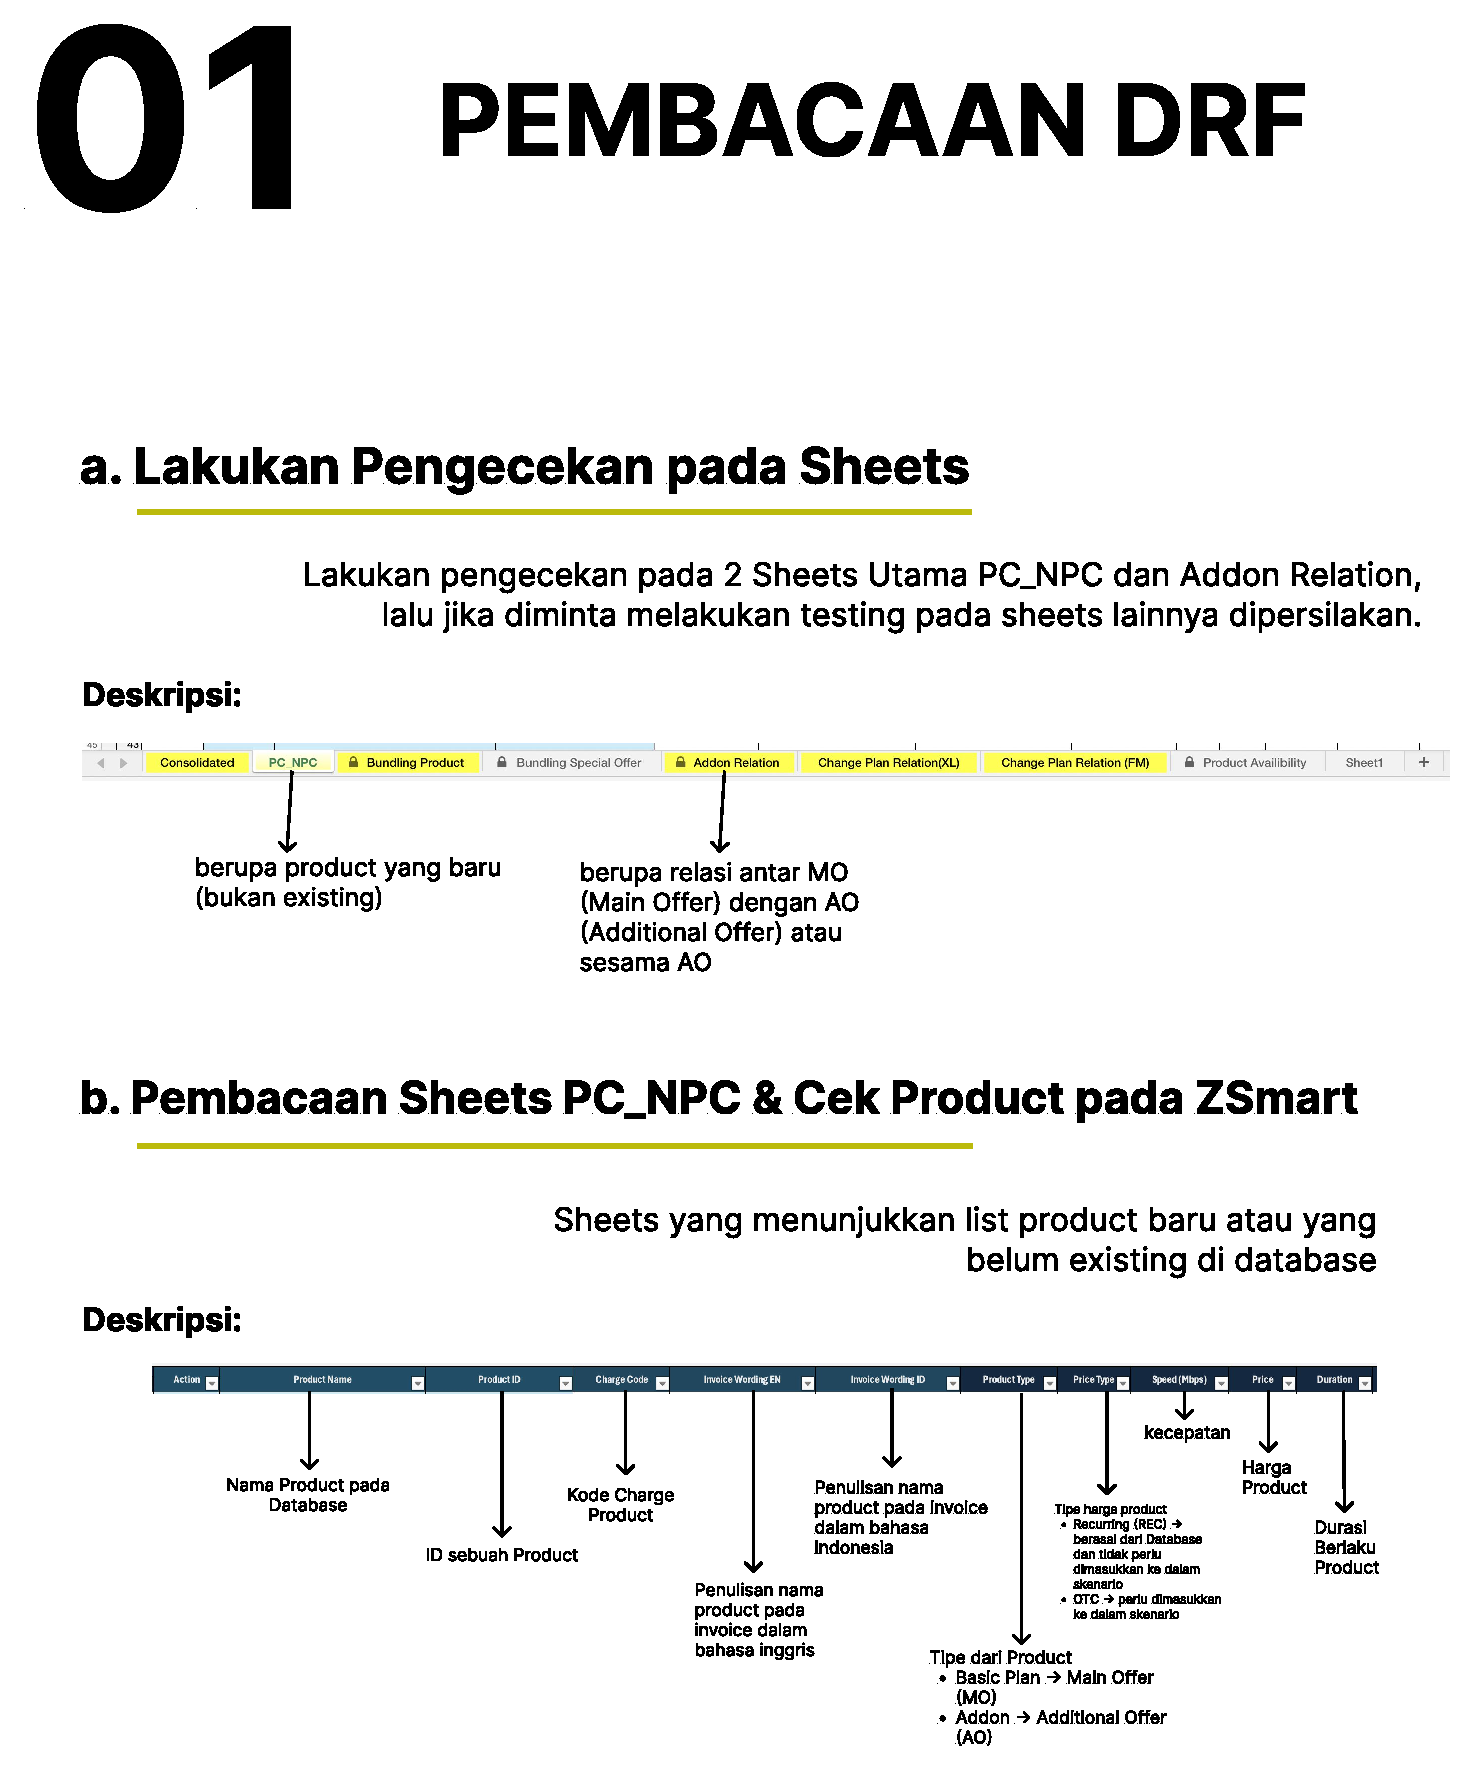
\includegraphics[width=0.92\textwidth]{gambar1_drf.png}
    \captionof{figure}{Bagian DRF yang digunakan untuk identifikasi produk dan relasi penawaran}
\end{center}

\vspace{0.4cm}
\noindent{\bfseries 3.3.2 Penyusunan Skenario Pengujian FTTH\par}
Skenario pengujian produk FTTH disusun menggunakan templat Microsoft Excel terstandar yang kompatibel dengan modul pengurai otomasi. Untuk pengujian aktivasi produk utama (MO), penulis menyusun lembar kerja bernama \textit{Activation MDN}. Parameter masukan utama terdiri atas: nomor akun uji pelanggan (MDN 8 digit), \textit{Product ID}, nama produk, dan kode siklus penagihan (\textit{billing cycle}). Parameter \textit{Product ID} dan penamaan diselaraskan secara presisi dengan lembar DRF guna menjaga ketertelusuran pengujian.

Nilai \textit{billing cycle} menentukan tanggal jatuh tempo perhitungan dan penerbitan faktur berkala. Sebagai contoh, untuk siklus penagihan tanggal 7 (BC07), pengujian yang dijalankan sebelum tanggal 8 akan diproses untuk faktur tanggal 8 bulan berjalan, sedangkan pengujian setelah tanggal 8 diarahkan pada siklus bulan berikutnya. Setelah variabel dilengkapi, baris \textit{header} teknis ditambahkan pada baris teratas agar format berkas dapat dikenali oleh kerangka otomasi Odoo. Pemetaan parameter DRF ke dalam skenario pengujian FTTH diilustrasikan pada Gambar 3.2.

\vspace{0.3cm}
\begin{center}
    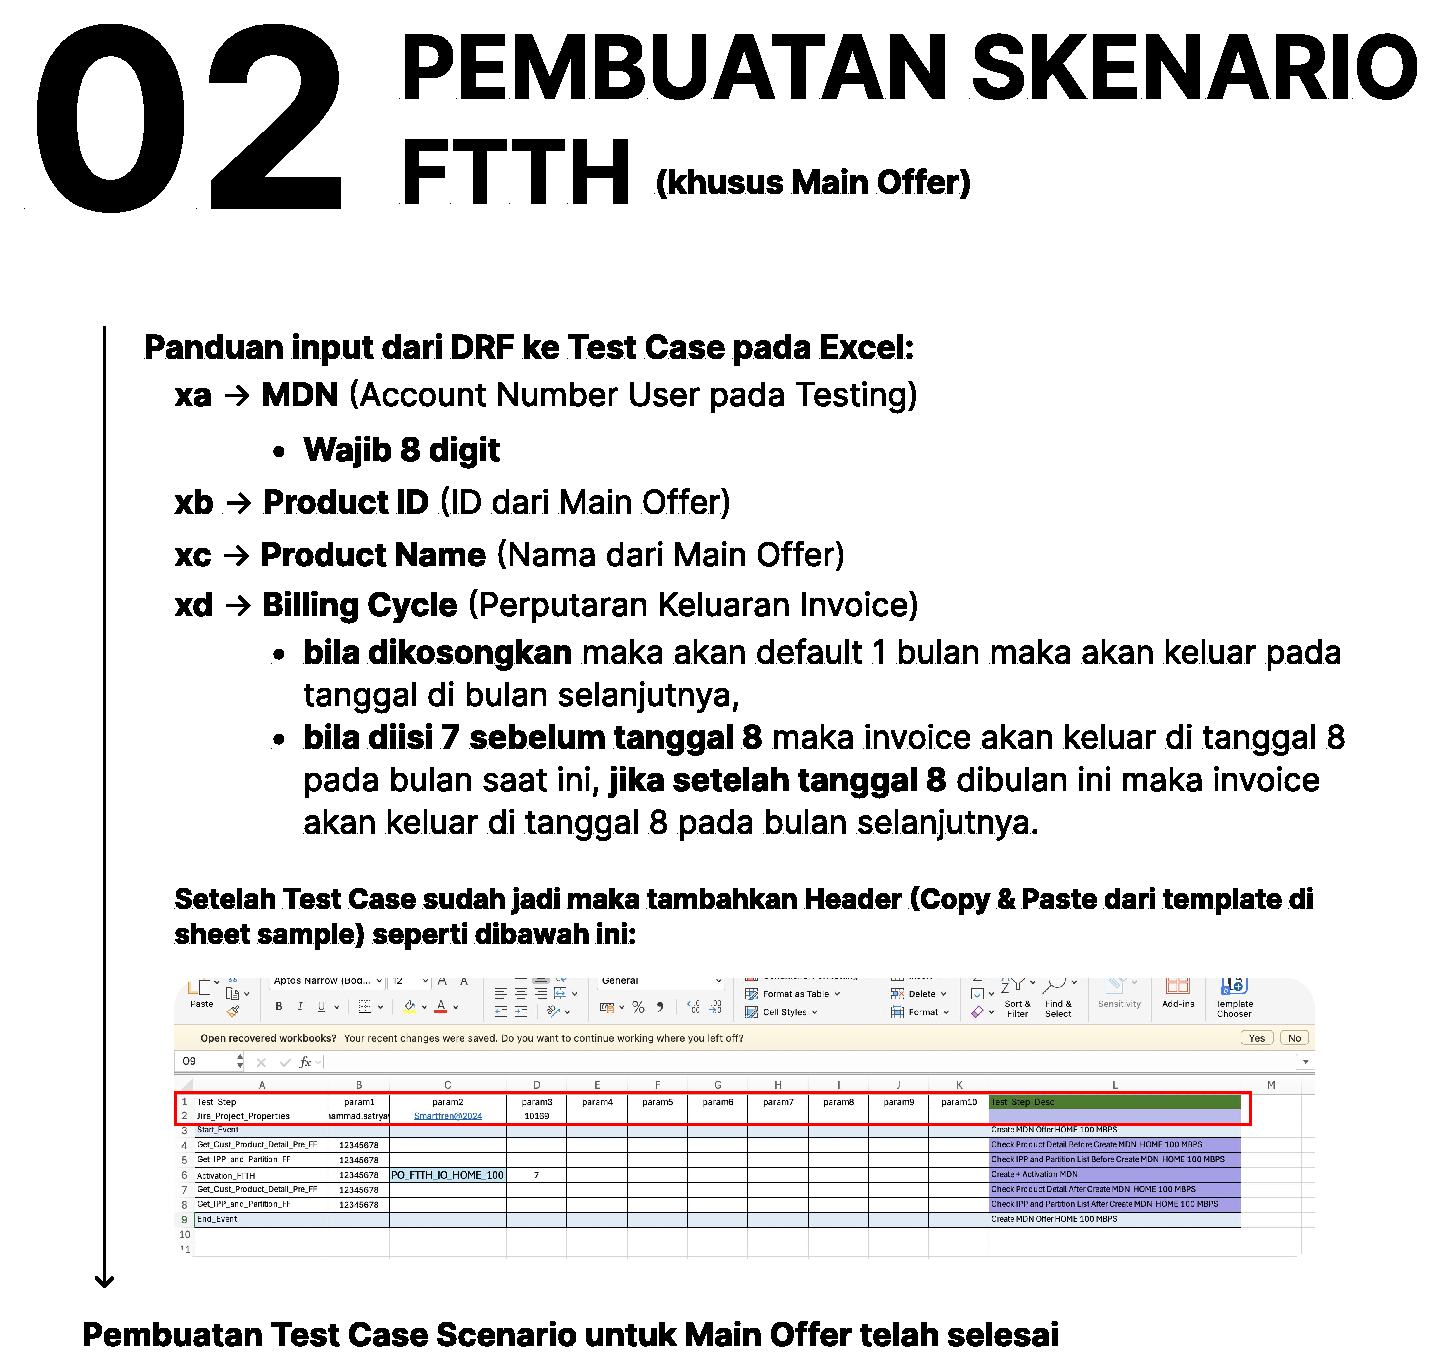
\includegraphics[width=0.92\textwidth]{gambar2_ftth.png}
    \captionof{figure}{Pemetaan parameter DRF ke skenario pengujian Main Offer FTTH}
\end{center}

Pengujian produk tambahan (AO) dikonfigurasikan pada lembar terpisah bernama \textit{Add AO} di dalam buku kerja yang sama. Setiap penambahan AO mensyaratkan keberadaan MO yang telah berstatus aktif pada nomor MDN yang bersangkutan. Parameter yang dicantumkan meliputi nomor MDN, \textit{Product ID} AO, nama AO, dan nominal harga. Apabila tipe penawaran adalah REC, kolom harga dibiarkan kosong karena sistem akan membaca langsung dari basis data katalog, sedangkan untuk tipe OTC, harga wajib diisi sesuai nominal pada DRF. Penulis juga merancang skenario uji negatif untuk memverifikasi penolakan sistem saat AO dipasangkan pada MO yang tidak kompatibel.

\vspace{0.4cm}
\noindent{\bfseries 3.3.3 Penyiapan Data dan Penyusunan Skenario Pengujian FWA\par}
Berbeda dengan produk FTTH yang hanya memerlukan alokasi nomor akun MDN virtual, pengujian varian nirkabel FWA menuntut penyiapan dan pengikatan identitas perangkat fisik telekomunikasi sebelum skenario uji dapat dieksekusi. Penulis menyiapkan empat berkas data pendukung berekstensi teks, yaitu \texttt{fwa.txt}, \texttt{iccid.txt}, \texttt{msisdn.txt}, dan \texttt{binding.txt}. Nomor ICCID dikumpulkan melalui menu \textit{SIM Profile Management} di ZSmart dengan memilih kartu SIM berstatus tersedia (\textit{available}) yang sesuai dengan profil FWA perusahaan. Sementara itu, nomor MSISDN diperoleh melalui menu \textit{MSISDN Profile} dengan memastikan statusnya belum terikat pada pelanggan mana pun.

Pasangan nomor ICCID dan MSISDN tersebut selanjutnya digabungkan ke dalam berkas \texttt{binding.txt}. Berkas ini diunggah ke sistem ZSmart melalui menu \textit{SIM \& MSISDN Binding/Unbinding} guna membentuk ikatan tunggal antara kartu fisik dan nomor layanan nirkabel, sebagaimana ditunjukkan pada Gambar 3.3. Pascapengikatan, penulis mengeksekusi rangkaian \textit{background batch jobs} (\textit{URF Batch}, \textit{PreNewConnection}, dan \textit{BatchNewConnection Job}) pada menu \textit{Wholesale Monitor} hingga status transaksi dinyatakan sukses. Proses diakhiri dengan membuka blokir ICCID (\textit{unblock ICCID}) dan menjalankan \textit{BatchBusiJob} agar profil SIM siap digunakan pada skenario aktivasi.

\vspace{0.3cm}
\begin{center}
    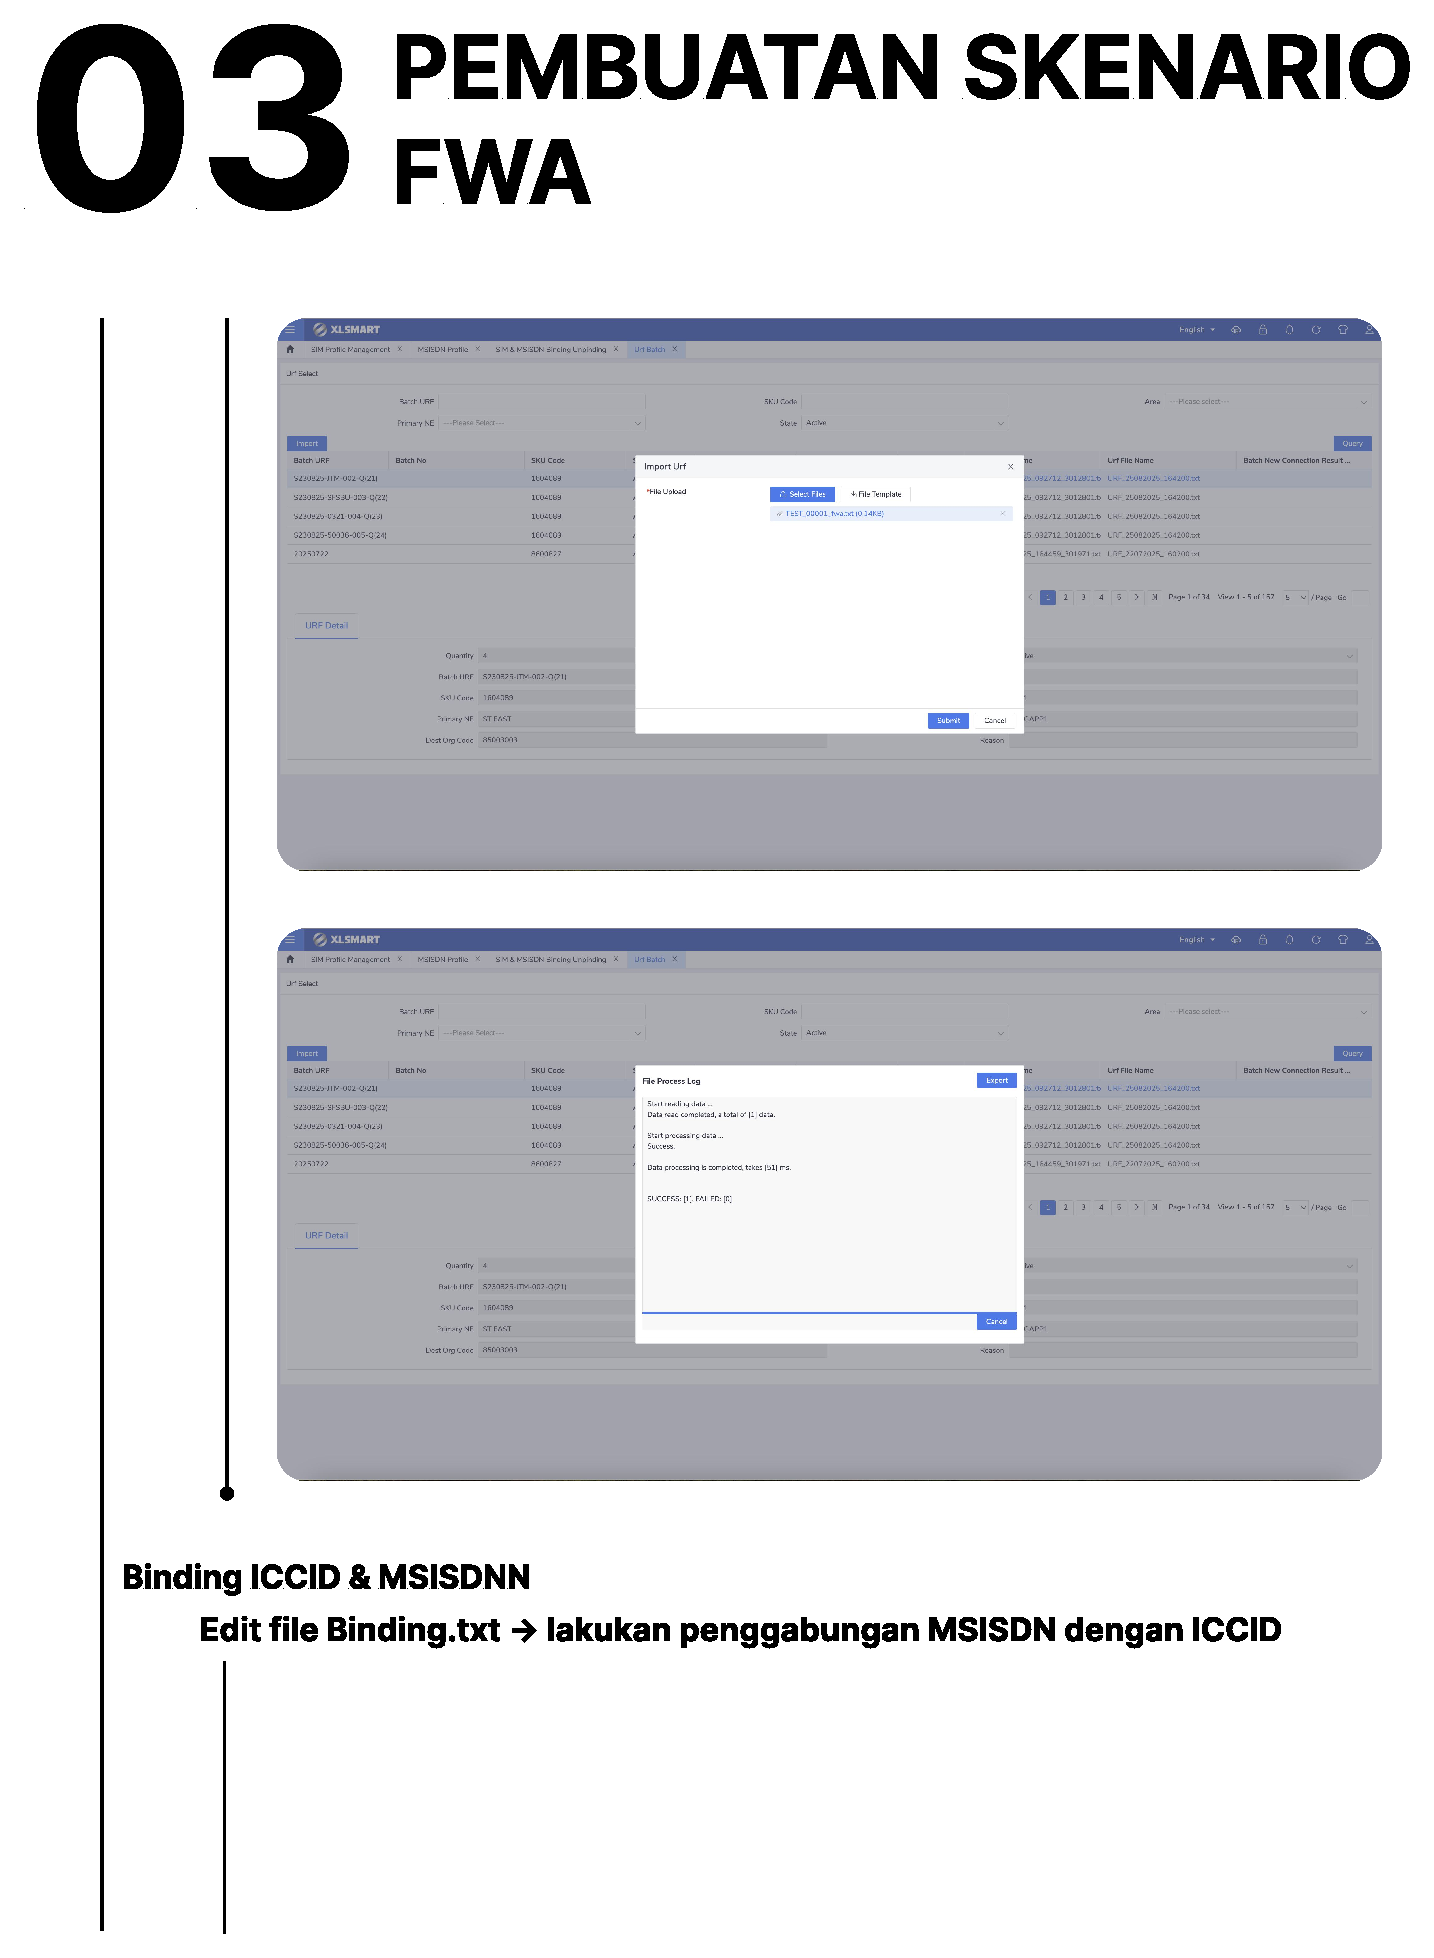
\includegraphics[width=0.92\textwidth]{gambar3_iccid.png}
    \captionof{figure}{Proses penggabungan ICCID dan MSISDN untuk penyiapan profil FWA}
\end{center}

Setelah profil identitas siap, penulis menyusun skenario aktivasi MO FWA pada berkas Excel dengan mencantumkan nomor MDN akun, \textit{Product ID}, nama paket, nomor MSISDN riil hasil pengikatan, serta kode siklus penagihan. Keberadaan nomor MSISDN riil ini merupakan pembeda fundamental dari skenario FTTH. Untuk pengujian produk tambahan AO FWA, skenario disusun pada lembar \textit{Add AO} dengan memastikan produk utama FWA telah aktif pada akun pelanggan. Contoh pemetaan variabel penawaran ke dalam skenario uji FWA diperlihatkan pada Gambar 3.4.

\vspace{0.3cm}
\begin{center}
    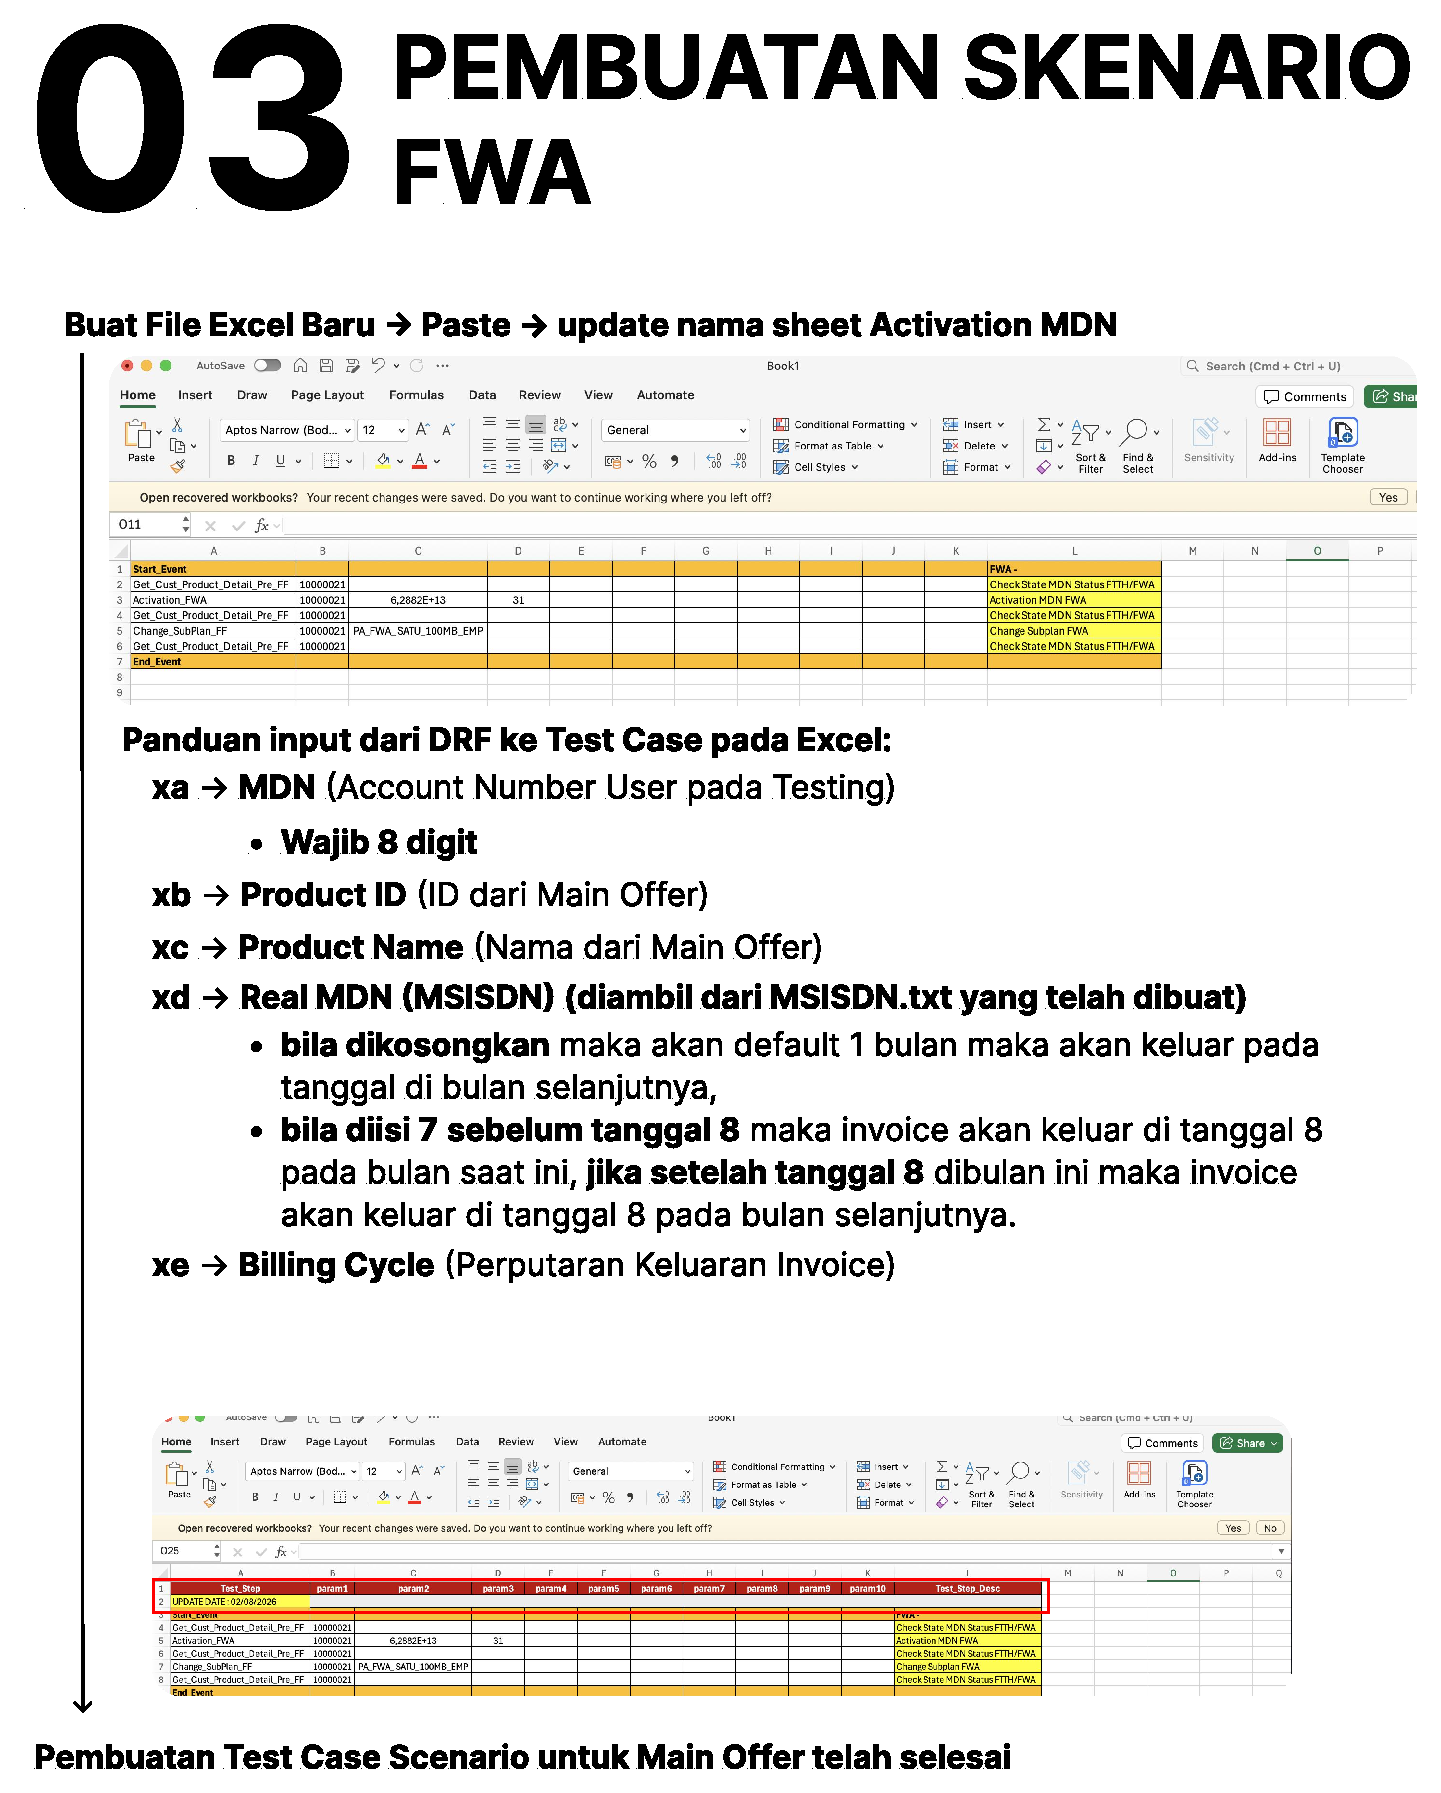
\includegraphics[width=0.92\textwidth]{gambar4_fwa.png}
    \captionof{figure}{Pemetaan data pelanggan dan produk ke skenario pengujian FWA}
\end{center}

\vspace{0.4cm}
\noindent{\bfseries 3.3.4 Pelaksanaan Run Recurring\par}
Setelah paket layanan berhasil diaktifkan pada sistem pengujian, penulis melanjutkan tahapan penjaminan mutu ke validasi siklus penagihan berkala melalui eksekusi \textit{run recurring}. Skenario ini bertujuan memverifikasi apakah sistem penagihan otomatis mampu memperpanjang masa aktif layanan dan membentuk pos biaya periode berikutnya secara akurat. Skenario disusun pada lembar kerja \textit{Recurring} dengan menginput nomor MDN akun dan parameter tanggal eksekusi yang ditargetkan.

Aturan penentuan tanggal eksekusi disesuaikan dengan siklus penagihan pelanggan. Untuk akun bersiklus akhir bulan (BC30), tanggal eksekusi diarahkan pada tanggal 1 bulan berikutnya. Sedangkan untuk siklus tanggal 7 (BC07), pengujian yang dijalankan sebelum tanggal 8 menggunakan tanggal 8 bulan berjalan, dan pengujian setelah tanggal 8 menggunakan tanggal 8 bulan berikutnya. Hasil eksekusi kemudian diperiksa pada basis data guna memastikan bahwa status layanan tetap aktif dan tagihan periode baru terbentuk tepat waktu. Struktur penyusunan skenario \textit{run recurring} ditunjukkan pada Gambar 3.5.

\vspace{0.3cm}
\begin{center}
    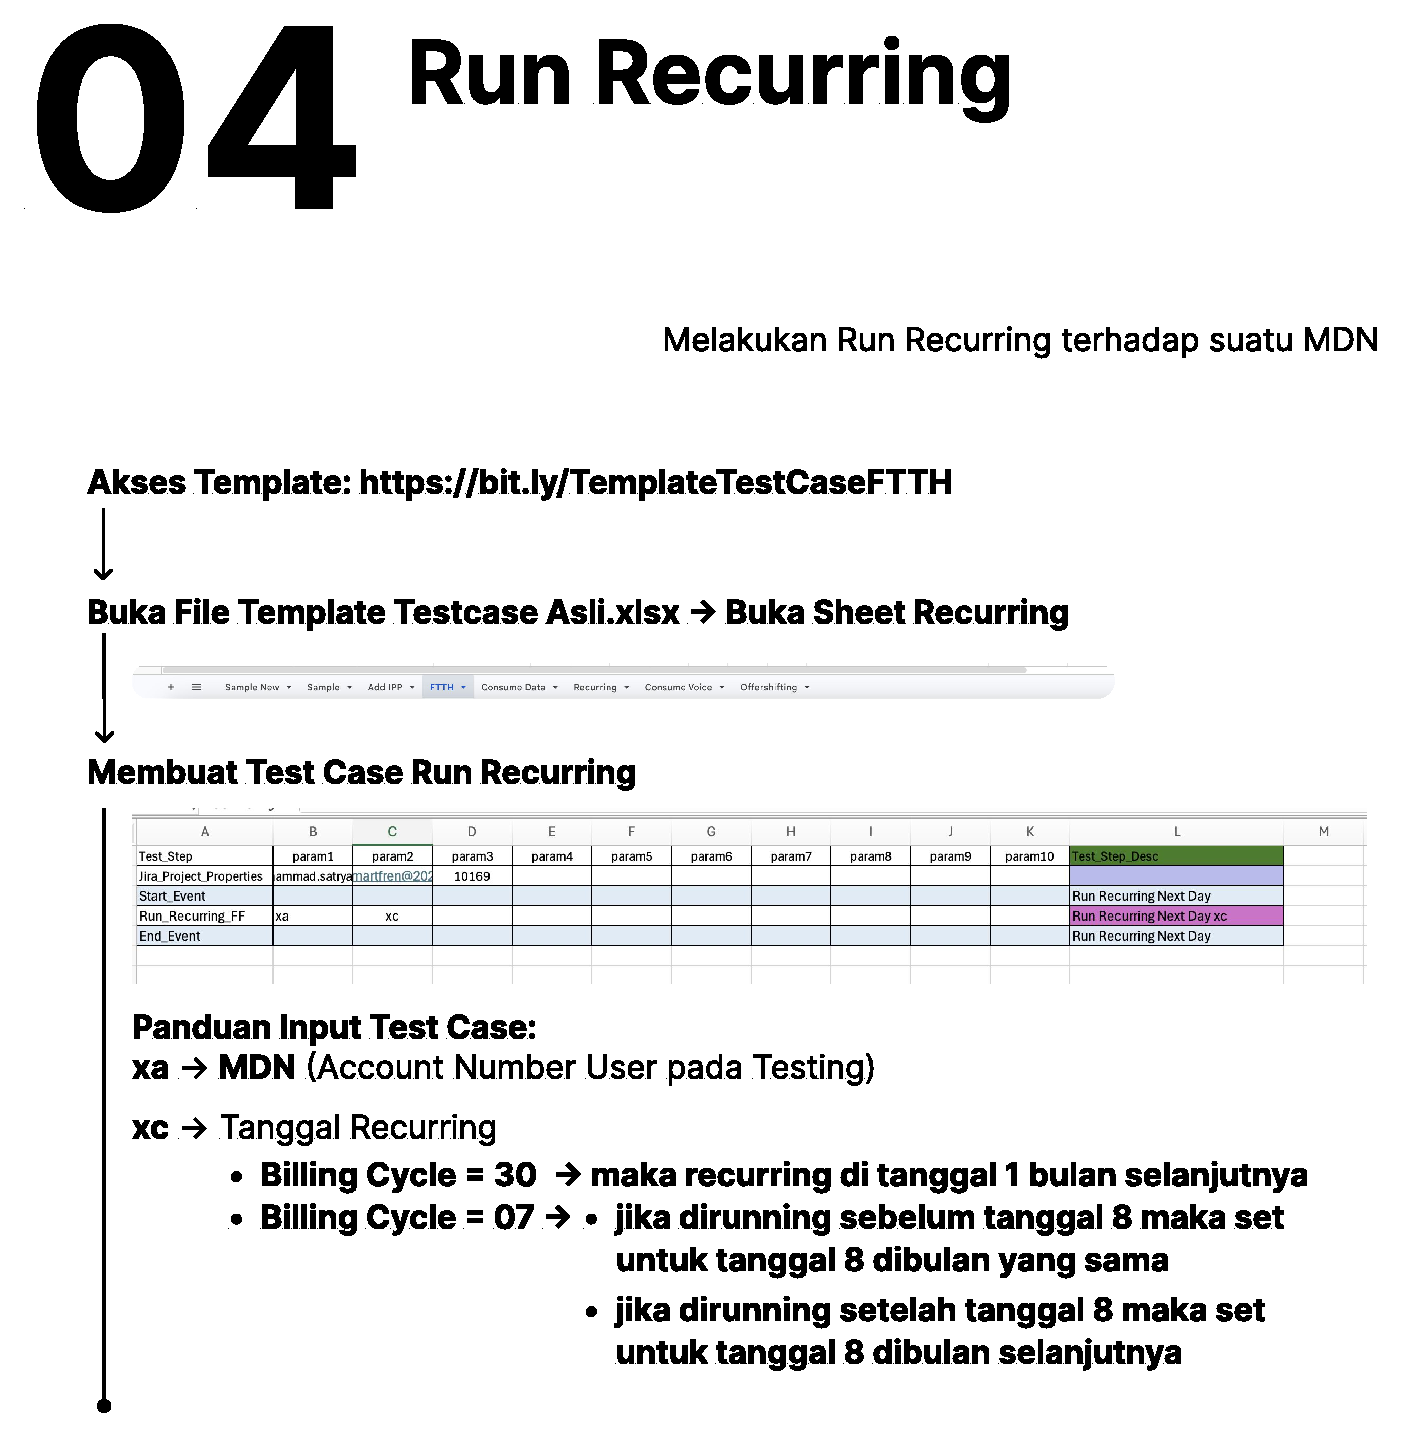
\includegraphics[width=0.92\textwidth]{gambar5_recurring.png}
    \captionof{figure}{Penyusunan skenario run recurring berdasarkan MDN dan billing cycle}
\end{center}

\vspace{0.4cm}
\noindent{\bfseries 3.3.5 Eksekusi Test Case melalui Odoo Automation\par}
Berkas kasus uji Excel yang telah terisi lengkap dieksekusi secara otomatis memanfaatkan platform Odoo Automation di lingkungan pengujian \textit{staging}. Penulis membuat entri skenario pengujian baru dengan menamainya sesuai nomor tiket DRF dan identitas produk yang diuji, lalu mengunggah berkas Excel terkait ke sistem. Setelah berkas berhasil terunggah, penulis menekan tombol \textit{Refresh Sheets} agar sistem mendeteksi seluruh lembar kerja di dalam berkas, memilih lembar uji yang akan dijalankan, lalu mengeksekusi perintah \textit{Parse Excel File}.

Proses penguraian (\textit{parsing}) mentransformasikan baris-baris data pada spreadsheet menjadi urutan panggilan antarmuka pemrograman (\textit{API calls}) ke sistem BSS secara otomatis. Penulis selanjutnya memulai eksekusi dan memantau progres langkah pengujian secara waktu-nyata (\textit{real-time}) melalui menu \textit{Test Executions}. Antarmuka Odoo Automation menyajikan log terperinci atas setiap tahapan yang berhasil dieksekusi maupun yang mengalami kegagalan, lengkap dengan pesan kesalahan dari server BSS. Alur pemilihan berkas, penguraian, dan pemantauan eksekusi di Odoo Automation ditunjukkan pada Gambar 3.6.

\vspace{0.3cm}
\begin{center}
    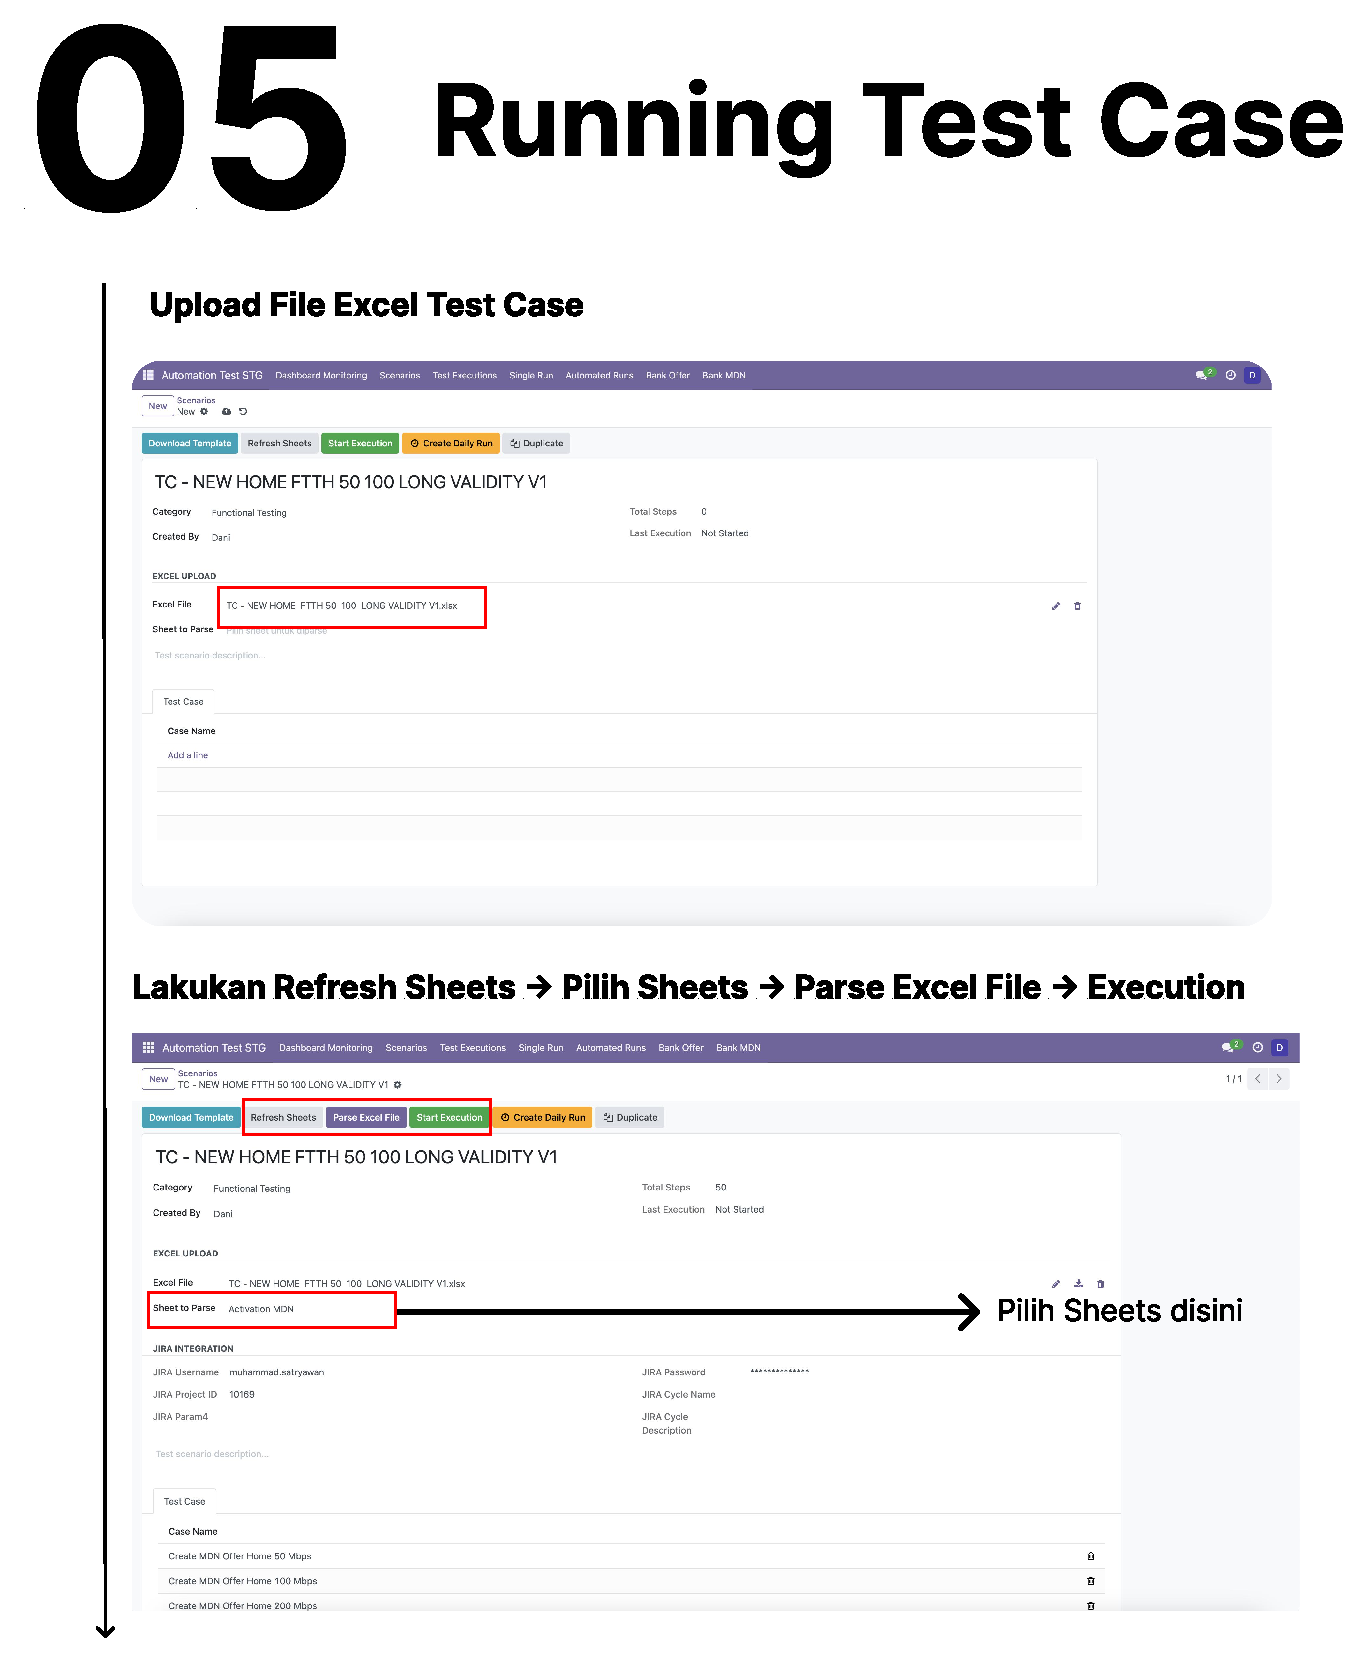
\includegraphics[width=0.92\textwidth]{gambar6_odoo.png}
    \captionof{figure}{Proses unggah, parsing, dan eksekusi test case pada Odoo Automation}
\end{center}

Setiap kegagalan eksekusi ditelaah secara kritis oleh penulis sebelum dilaporkan sebagai \textit{defect}. Penulis membedakan apakah kegagalan disebabkan oleh ketidaksesuaian logika produk murni, data identitas SIM/MDN yang kedaluwarsa, gangguan pada antrean sistem ZSmart, atau galat sintaks pada berkas skenario. Temuan yang terkonfirmasi sebagai cacat konfigurasi produk didokumentasikan beserta langkah reproduksi dan bukti log transaksi untuk dibahas bersama tim pengembang dan mentor.

\vspace{0.4cm}
\noindent{\bfseries 3.3.6 Mock Bill Check dan Validasi Invoice\par}
Tahap krusial berikutnya dalam rangkaian penjaminan mutu penagihan adalah pelaksanaan simulasi faktur (\textit{mock bill check}). Tahap ini memverifikasi bahwa produk yang telah aktif dan mengalami perpanjangan siklus menghasilkan rincian komponen tagihan yang benar-benar akurat sesuai klausul pada dokumen DRF. Penulis mengakses menu \textit{Mock Bill Entry} pada aplikasi ZSmart, memasukkan nomor MDN akun yang diuji, dan memicu kalkulasi simulasi penagihan.

Hasil simulasi selanjutnya dibuka melalui menu \textit{Mock Bill Inquiry}, di mana berkas rincian faktur diunduh untuk dianalisis baris demi baris. Penulis memeriksa kesesuaian nama produk yang tercetak, kurun waktu penagihan, kode biaya, besaran nominal sebelum pajak, perhitungan pajak pertambahan nilai, serta total akhir tagihan. Produk bertipe REC wajib tercantum pada kategori biaya berulang, sedangkan produk bertipe OTC hanya boleh muncul sebagai biaya sekali bayar pada faktur pertama. Langkah verifikasi ini berhasil mencegah anomali kesalahan pemotongan saldo pelanggan, duplikasi biaya tagihan, maupun ketidaksesuaian teks faktur komersial. Tampilan pemeriksaan komponen penagihan pada hasil \textit{mock bill} diperlihatkan pada Gambar 3.7.

\vspace{0.3cm}
\begin{center}
    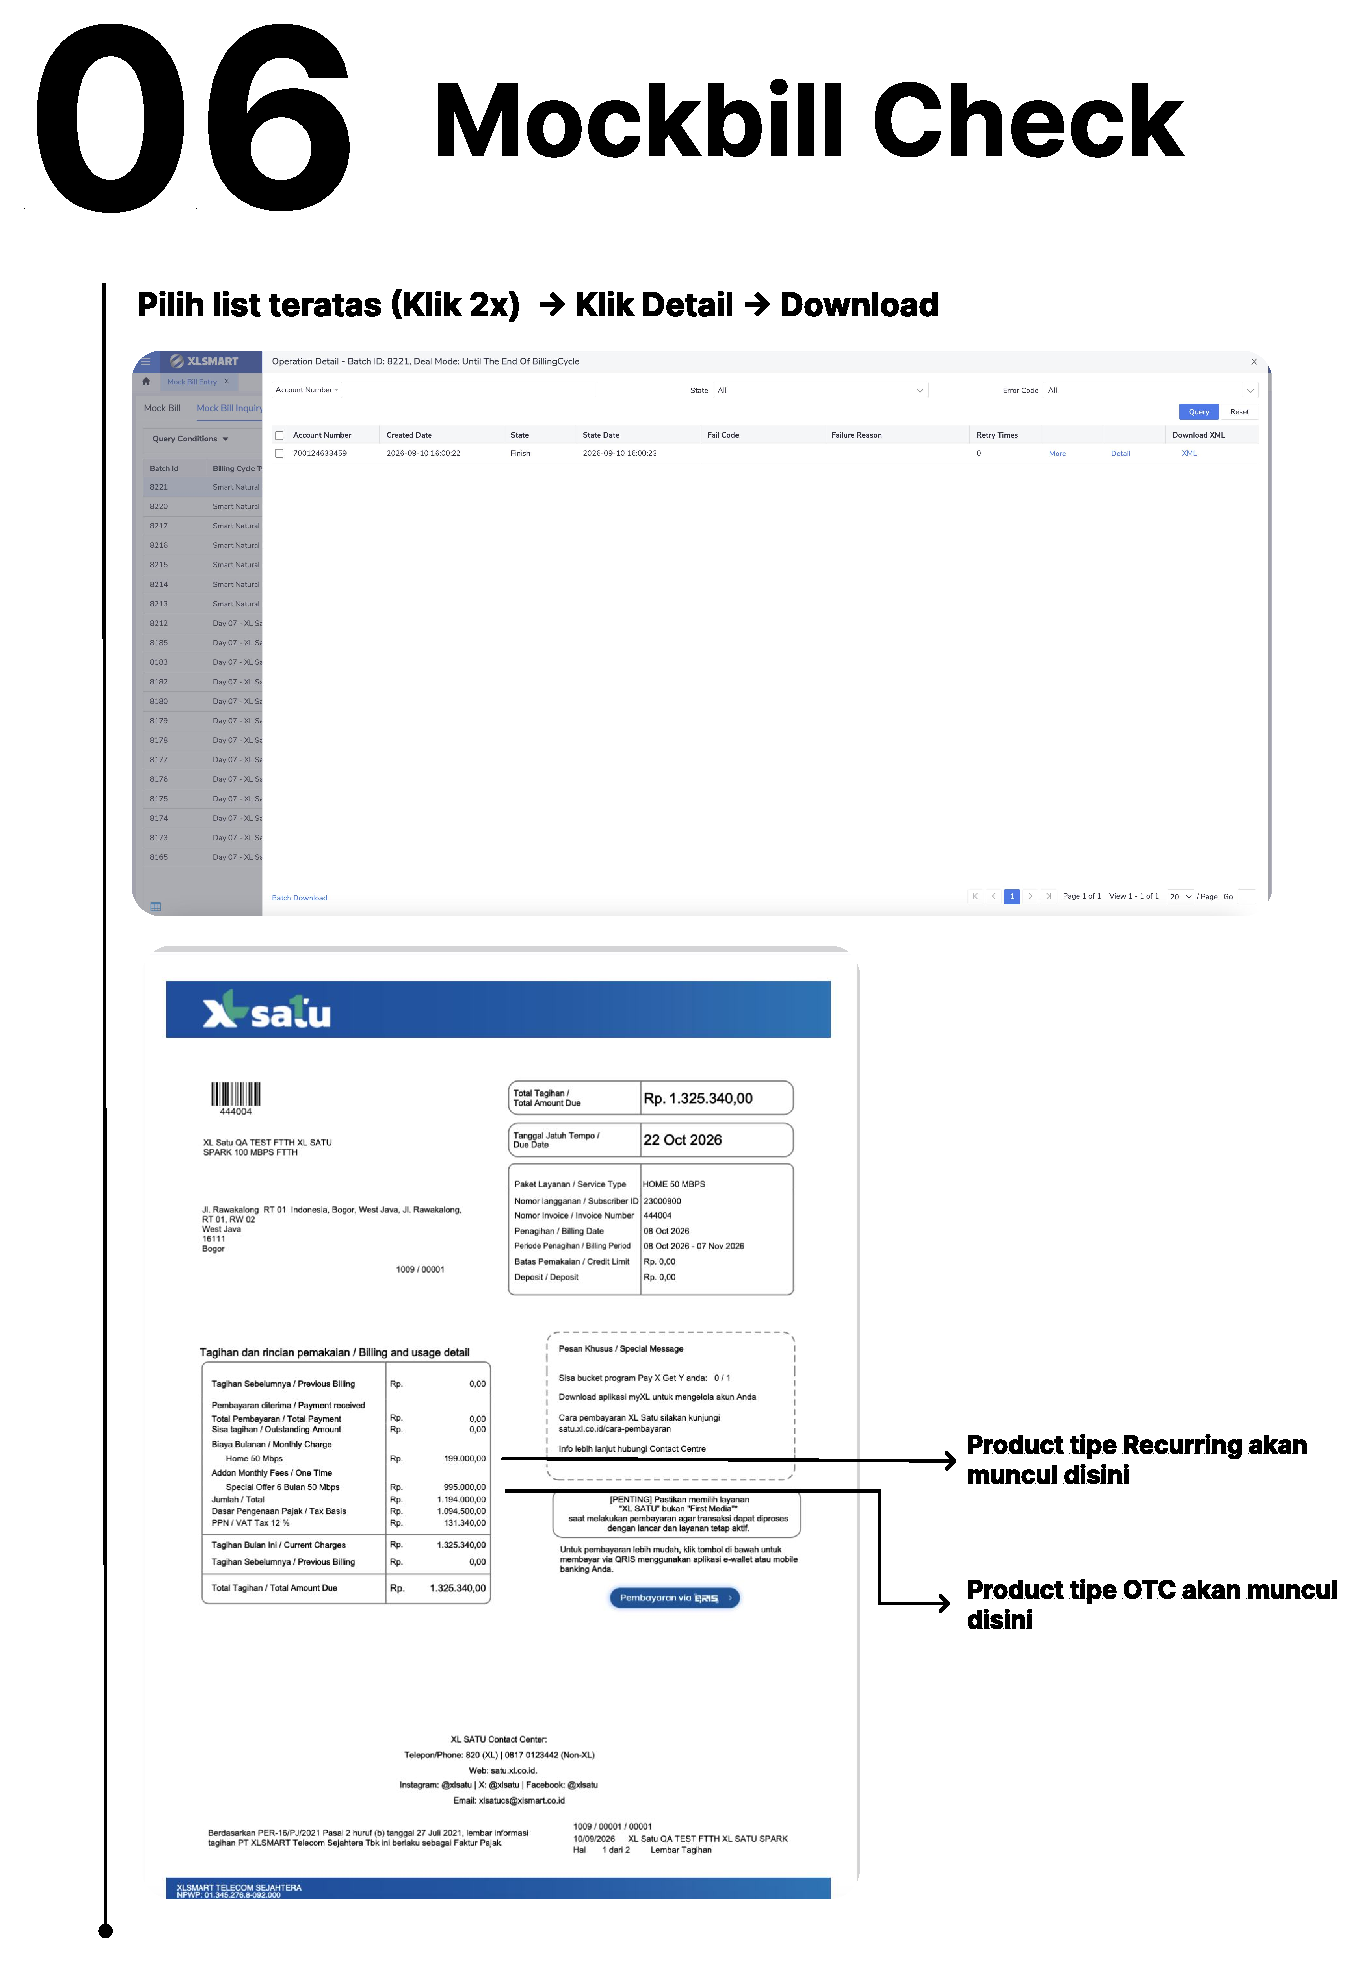
\includegraphics[width=0.92\textwidth]{gambar7_mockbill.png}
    \captionof{figure}{Pemeriksaan komponen recurring dan OTC pada hasil mock bill}
\end{center}

\vspace{0.4cm}
\noindent{\bfseries 3.3.7 Verifikasi Hasil dan Dokumentasi Pendukung\par}
Sebagai tahap konfirmasi akhir, penulis melakukan verifikasi menyeluruh terhadap akun pelanggan menggunakan modul-modul pendukung pada sistem ZSmart. Menu \textit{Account Receivable} digunakan untuk menelusuri riwayat transaksi penagihan dan memastikan status pembayaran tagihan tercatat lunas tanpa menyisakan saldo piutang tertunggak yang tidak wajar. Sementara itu, menu \textit{Order Entry} dibuka guna memeriksa inventaris produk yang terpasang pada akun, memastikan bahwa status indikator produk utama (MO) dan produk tambahan (AO) berada dalam status aktif (\textit{active}) dengan parameter teknis yang tepat. Contoh tampilan verifikasi akun dan riwayat transaksi penagihan ditunjukkan pada Gambar 3.8.

\vspace{0.3cm}
\begin{center}
    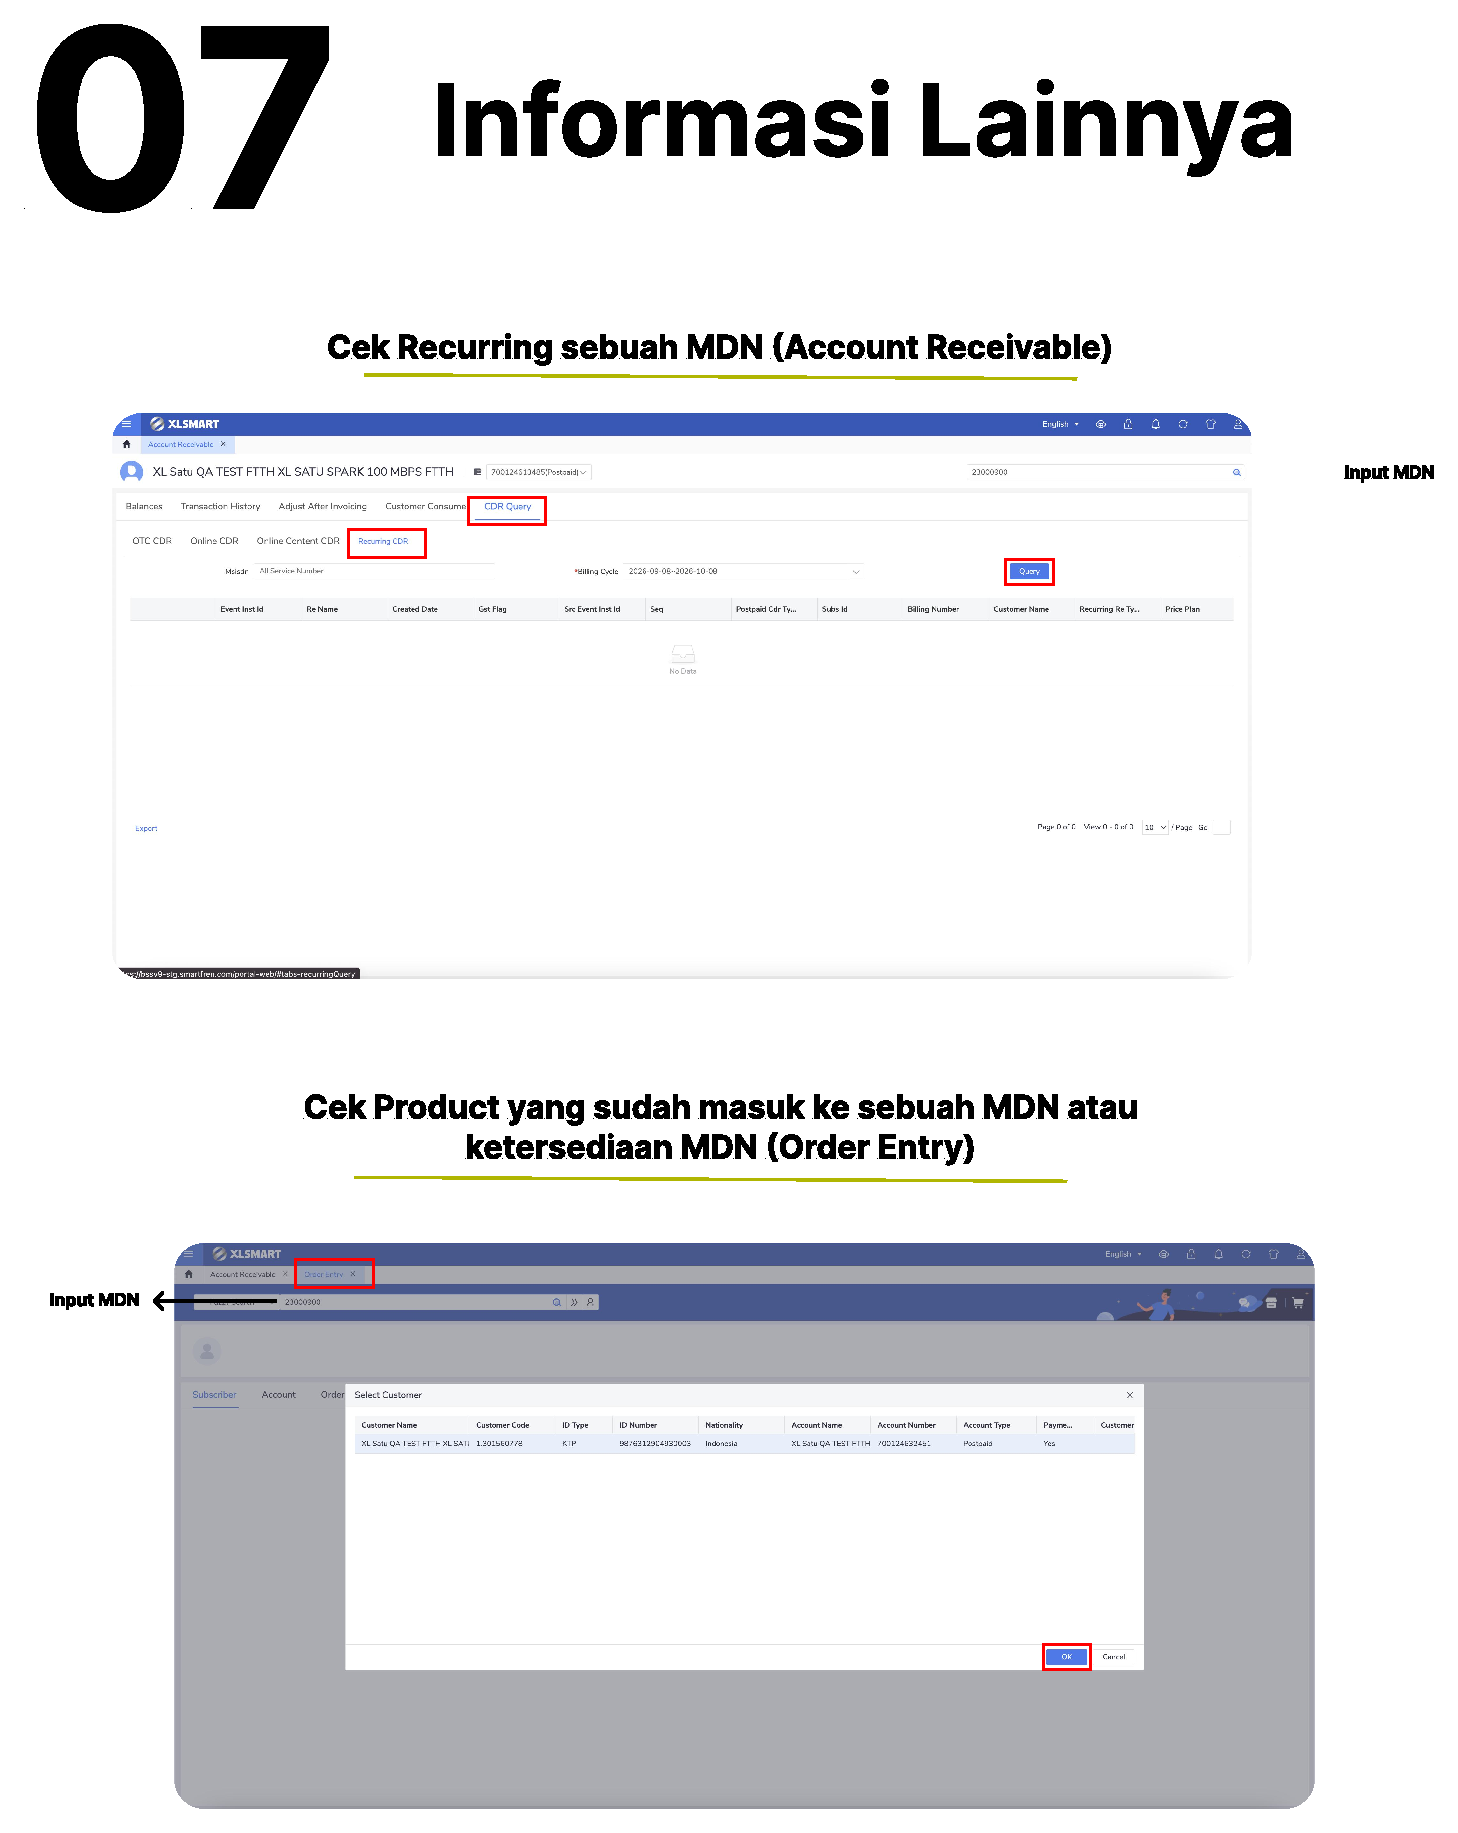
\includegraphics[width=0.92\textwidth]{gambar8_verification.png}
    \captionof{figure}{Verifikasi recurring dan produk pelanggan melalui Account Receivable dan Order Entry}
\end{center}

Apabila ditemukan inkonsistensi kalkulasi tagihan selama pengujian, penulis memanfaatkan fungsi \textit{Billing Redo} atau \textit{Ledger} pada ZSmart untuk membatalkan dan mengulang kalkulasi penagihan sesuai siklus akun yang diuji (misalnya siklus hari ke-7 untuk BC07 atau akhir bulan untuk BC31). Penulis mengambil nomor identifikasi langganan (\textit{SUBSID}) dari hasil eksekusi Odoo Automation atau kueri basis data DBeaver untuk melacak rekonsiliasi data penagihan. Seluruh bukti hasil uji, tangkapan layar verifikasi, dan status kelulusan tiket dicatat pada sistem dokumentasi internal tim. Setelah perbaikan konfigurasi diterapkan oleh tim pengembang, penulis menjalankan pengujian regresi ulang (\textit{re-testing}) guna memastikan seluruh alur transaksi telah berfungsi sempurna tanpa memicu efek samping pada modul penagihan lainnya.

% ==================== BAB IV: PENUTUP ====================
\clearpage
\begin{center}
    {\bfseries\large BAB IV\par}
    {\bfseries\large PENUTUP\par}
\end{center}
\vspace{0.4cm}

\noindent{\bfseries 4.1 Kesimpulan\par}
Berdasarkan pelaksanaan kegiatan Kerja Praktik sebagai \textit{Quality Assurance Automation Engineer} pada unit IT Core Charging PT XLSMART Telecom Sejahtera Tbk selama periode 29 Juni 2026 hingga 15 September 2026, dapat ditarik beberapa kesimpulan utama sebagai berikut:
\begin{enumerate}[label=\arabic*.,leftmargin=1.5em,itemsep=3pt,topsep=2pt]
    \item \textbf{Efektivitas Analisis Kebutuhan Katalog Produk:} Proses telaah dokumen DRF (\textit{Document Request Form}) dan validasi konfigurasi katalog penawaran pada ZSmart (CPC Manager) terbukti menjadi fondasi krusial dalam menyusun skenario kasus uji yang akurat. Pemahaman mendalam mengenai dekomposisi produk utama (\textit{Main Offer}), produk tambahan (\textit{Additional Offer}), tipe biaya (REC/OTC), serta relasi dependensi berhasil memastikan bahwa skenario pengujian merepresentasikan logika bisnis produk FTTH dan FWA secara tepat.
    \item \textbf{Peningkatan Efisiensi Pengujian melalui Otomasi:} Penerapan pengujian berbasis data (\textit{Data-Driven Testing}) menggunakan kerangka Odoo Automation berhasil meningkatkan efisiensi waktu eksekusi kasus uji berulang secara signifikan dibandingkan metode manual murni. Pemisahan antara data uji pada spreadsheet Excel dan logika eksekusi sistem memungkinkan pengujian terhadap puluhan permutasi produk broadband dijalankan secara konsisten dan akurat.
    \item \textbf{Validasi End-to-End Siklus Penagihan Pelanggan:} Penjaminan mutu berhasil diperluas tidak hanya pada tahap aktivasi awal layanan, melainkan hingga tahap pembaruan siklus penagihan otomatis (\textit{run recurring}) dan simulasi faktur (\textit{mock bill check}). Validasi komponen biaya berulang (REC) dan biaya sekali bayar (OTC) berhasil mencegah potensi kesalahan penetapan tarif serta melindungi jutaan pelanggan dari anomali pembukuan tagihan.
    \item \textbf{Penerapan Etika Profesi dan Budaya Kolaborasi Industri:} Penulis berhasil menerapkan prinsip etika rekayasa perangkat lunak melalui pelaporan \textit{defect} yang objektif berbasis bukti, menjaga kerahasiaan data uji korporat secara ketat melalui jaringan VPN berizin, serta membangun komunikasi profesional yang harmonis bersama mentor lapangan, pengembang, dan sesama penguji di lingkungan kerja berkecepatan tinggi.
    \item \textbf{Penyusunan Warisan Dokumentasi Pengetahuan Baku:} Kegiatan Kerja Praktik berhasil menghasilkan luaran konkret berupa Buku Panduan Testing FTTH/FWA sebagai dokumentasi acuan operasional resmi bagi unit IT Core Charging, yang membakukan tata cara penyiapan data kartu SIM, penyusunan berkas skenario, eksekusi otomasi, hingga verifikasi faktur bagi kelangsungan pengujian tim di masa depan.
\end{enumerate}

\vspace{0.4cm}
\noindent{\bfseries 4.2 Saran\par}
Sebagai upaya perbaikan dan pengembangan berkelanjutan bagi pelaksanaan pengujian perangkat lunak di masa mendatang, penulis menyampaikan beberapa saran konstruktif:
\begin{enumerate}[label=\arabic*.,leftmargin=1.5em,itemsep=3pt,topsep=2pt]
    \item \textbf{Pengembangan Lingkungan Uji Mandiri (Sandbox TDM):} Unit kerja disarankan menyediakan sistem \textit{Test Data Management} (TDM) terotomasi yang mampu mengalokasikan dan melepaskan pasangan nomor kartu ICCID dan MSISDN uji secara instan, guna memangkas waktu penyiapan data identitas FWA sebelum pengujian dimulai.
    \item \textbf{Integrasi Otomasi Asersi Faktur (Automated Mock Bill Assertion):} Proses pemeriksaan hasil \textit{mock bill} yang saat ini sebagian besar masih ditelaah secara visual disarankan untuk diintegrasikan dengan modul pembanding otomatis (\textit{automated diff assertion}) di dalam Odoo Automation, sehingga disparitas komponen harga dapat terdeteksi secara otomatis oleh sistem.
    \item \textbf{Pemeliharaan Berkelanjutan Buku Panduan Pengujian:} Dokumentasi Buku Panduan Testing FTTH/FWA hendaknya diperbarui secara berkala di repositori internal perusahaan setiap kali terdapat penambahan modul BSS baru atau perubahan arsitektur katalog produk pascamerger.
    \item \textbf{Bagi Mahasiswa Peserta Kerja Praktik Berikutnya:} Mahasiswa disarankan memperkuat penguasaan konsep relasi basis data enterprise (kueri SQL transaksi), memahami arsitektur sistem penagihan telekomunikasi (\textit{charging and billing lifecycle}), serta mengasah kedisiplinan pencatatan bukti uji sejak awal penugasan di industri.
\end{enumerate}

% ==================== DAFTAR PUSTAKA ====================
\clearpage
\begin{center}
    {\bfseries\large DAFTAR PUSTAKA\par}
\end{center}
\vspace{0.6cm}

\noindent
\begin{enumerate}[label={[\arabic*]},leftmargin=2.2em,itemsep=6pt,topsep=2pt]
    \item ANTARA News, ``XL Axiata dan Smartfren resmi merger menjadi XLSmart,'' Jakarta, Indonesia, 2025. [Daring]. Tersedia: \url{https://www.antaranews.com/berita/4735701/xl-axiata-dan-smartfren-resmi-merger-menjadi-xlsmart}. Diakses: 28 September 2026.
    \item M. Fewster dan D. Graham, \textit{Software Test Automation: Effective Use of Test Execution Tools}. Harlow, Inggris: Addison-Wesley, 1999.
    \item International Software Testing Qualifications Board, ``Certified Tester Foundation Level Syllabus v4.0.1,'' ISTQB, 15 September 2024. [Daring]. Tersedia: \url{https://istqb.org/wp-content/uploads/2024/11/ISTQB_CTFL_Syllabus_v4.0.1.pdf}. Diakses: 28 September 2026.
    \item D. Graham dan M. Fewster, \textit{Experiences of Test Automation: Case Studies of Software Test Automation}. Upper Saddle River, NJ: Addison-Wesley, 2012.
    \item ACM/IEEE-CS Joint Task Force on Software Engineering Ethics and Professional Practices, ``Software Engineering Code of Ethics and Professional Practice, Version 5.2,'' Association for Computing Machinery dan IEEE Computer Society, 1999.
    \item K. Schwaber dan J. Sutherland, ``The Scrum Guide: The Definitive Guide to Scrum,'' November 2020. [Daring]. Tersedia: \url{https://scrumguides.org/docs/scrumguide/v2020/2020-Scrum-Guide-US.pdf}. Diakses: 28 September 2026.
    \item B. W. Tuckman, ``Developmental sequence in small groups,'' \textit{Psychological Bulletin}, vol. 63, no. 6, pp. 384--399, 1965.
    \item \textit{Software and Systems Engineering---Software Testing---Part 1: General Concepts}, ISO/IEC/IEEE 29119-1:2022, 2022.
    \item \textit{Systems and Software Engineering---Life Cycle Processes---Requirements Engineering}, ISO/IEC/IEEE 29148:2018, 2018.
    \item TM Forum, ``TMF620 Product Catalog Management API, Version 5.0.0,'' TM Forum Open API. [Daring]. Tersedia: \url{https://www.tmforum.org/open-digital-architecture/open-apis/product-catalog-management-api-TMF620/v5.0}. Diakses: 28 September 2026.
    \item 3rd Generation Partnership Project, ``Characteristics of the Universal Subscriber Identity Module (USIM) Application,'' 3GPP TS 31.102, Release 18, 2025.
    \item Odoo S.A., ``Subscriptions,'' Odoo 19.0 Documentation, 2026. [Daring]. Tersedia: \url{https://www.odoo.com/documentation/19.0/applications/sales/subscriptions.html}. Diakses: 28 September 2026.
    \item TM Forum, ``TMF678 Customer Bill Management API, Version 5.0.0,'' TM Forum Open API, 8 Mei 2026. [Daring]. Tersedia: \url{https://www.tmforum.org/open-digital-architecture/open-apis/customer-bill-management-api-TMF678/v5.0}. Diakses: 28 September 2026.
    \item \textit{Information Security, Cybersecurity and Privacy Protection---Information Security Management Systems---Requirements}, ISO/IEC 27001:2022, International Organization for Standardization, 2022.
\end{enumerate}

% ==================== LAMPIRAN ====================
\clearpage
\begin{center}
    {\bfseries\large LAMPIRAN\par}
\end{center}
\vspace{0.4cm}

\noindent\textbf{Lampiran 1: Dokumentasi Kegiatan Kerja Praktik}\par
\vspace{0.2cm}
\noindent Lembar dokumentasi kegiatan operasional Kerja Praktik di PT XLSMART Telecom Sejahtera Tbk (Unit IT Core Charging), XLSMART Tower, Jakarta Selatan. Foto-foto dokumentasi resmi kegiatan disiapkan pada bingkai dokumentasi berikut:

\vspace{0.4cm}
\begin{center}
    \begin{tabular}{|p{14.0cm}|}
    \hline
    \vspace{1.2cm}
    \begin{center}
        \textit{[Ruang Dokumentasi Foto Kegiatan 1: Lingkungan Kerja \& Fasilitas Pengujian IT Core Charging, XLSMART Tower]}
    \end{center}
    \vspace{1.2cm}
    \\
    \hline
    \end{tabular}
\end{center}

\vspace{0.4cm}
\begin{center}
    \begin{tabular}{|p{14.0cm}|}
    \hline
    \vspace{1.2cm}
    \begin{center}
        \textit{[Ruang Dokumentasi Foto Kegiatan 2: Koordinasi Tim Penguji, Weekly Sprint Sync, \& Sesi Transfer Pengetahuan]}
    \end{center}
    \vspace{1.2cm}
    \\
    \hline
    \end{tabular}
\end{center}

\clearpage
\begin{center}
    \begin{tabular}{|p{14.0cm}|}
    \hline
    \vspace{1.5cm}
    \begin{center}
        \textit{[Ruang Dokumentasi Foto Kegiatan 3: Presentasi Akhir Capaian Pengujian \& Seremoni Pelepasan Kerja Praktik]}
    \end{center}
    \vspace{1.5cm}
    \\
    \hline
    \end{tabular}
\end{center}

\vspace{0.8cm}
\noindent\textbf{Lampiran 2: Tautan Repositori Video Dokumentasi Kegiatan}\par
\vspace{0.3cm}
\noindent Seluruh rekaman video kegiatan harian, pembuktian eksekusi otomasi pengujian, dan rangkuman aktivitas Kerja Praktik telah diunggah dan dapat diakses pada repositori penyimpanan awan resmi melalui tautan berikut:\par
\vspace{0.2cm}
\noindent\url{https://drive.google.com/drive/folders/1bBYJVn4oPF5wOKXdknpi9M7JqReDMrfQ}

\end{document}